\documentclass[hyperref,bachelorofscience,fleqn]{cgvpub}
%weitere Optionen zum Ergänzen (in eckigen Klammern):
% 
% bibnum	numerische Literaturschlüssel
% final 	für Abgabe	
% lof			Abbildungsverzeichis
% lot			Tabellenverzeichnis
% noproblem	keine Aufgabenstellung
% notoc			kein Inhaltsverzeichnis
% twoside		zweiseitig
\author{Adrian Bielefeldt}
\title{Title}
\birthday{15. October 1994}
\placeofbirth{Dresden}
\matno{3694323}
\betreuer{Prof. Dr. Markus Kr{\"{o}}tzsch}
\bibfiles{literatur}
\problem{problem}
\copyrighterklaerung{copyright stuff}
\acknowledgments{Acknowledgements}
\abstracten{abstract text English}

\usepackage{rotating}
\usepackage{float}
\restylefloat{table}
\usepackage{makecell}
\renewcommand{\cellalign}{tl}
\usepackage{tabularx}
\usepackage{todonotes}
\usepackage{adjustbox}
\usepackage[shortlabels]{enumitem}
\usepackage{graphicx}
\usepackage{amsthm}

\setcounter{tocdepth}{2}

\newtheorem{example}{Example}


\begin{document}
\chapter{Introduction}
Wikidata, the knowledge base sister project of Wikipedia, has grown to be one of the most used open data resources available on the web. Wikidata is closely integrated with Wikipedia, where it links pages across languages and provides language-independent content (such as birth dates or population figures). Additionally, several services outside of the Wikimedia make use of Wikidata.  Probably the best-known example is the knowledge graph by Google, shown in information boxes to the right or top of search results on their main page. These facts are sourced from a variety of databases, Wikidata among them. Openstreetmap links objects with a physical presence to its Wikidata pages (and vice versa). \todo{more examples, if they can be found}

As of September 2018, Wikidata contains more than 50 million pages with over 500 million statements. More than 34.000 contributors worked on Wikidata in August 2018 alone, and more than 18.4 million facts where edited or created. Multiple open data collections are linked through Wikidata, such as VIAF, DOI, or BBC Programmes. More on the structure of Wikidata is explained in Section \ref{sec_wikidata}.

Because of Wikidatas widespread usage and frequent editing, it is necessary to ensure the correctness and quality of the data. Mechanisms to support data quality are, among others, referencing the sources of statements, cross-checking by the community, and constraints.

Constraints limit how the content of Wikidata may related to itself. Some facts can be in conflict with others, meaning one of the two is in all likelihood wrong. Other facts can require certain facts to be stated in the database as well, thus pointing to data that may be missing. Constraints are used to ensure data correctness as well as clarify the data structure in cases where it might be unclear how facts should be described. A detailed explanation of these constrains can be found
in Chapter \ref{cha_property_constraints}.

Since Wikidata is a very large and constantly changing resource, it is necessary to find ways to quickly and efficiently determine violations of these constraints. One solution offering itself are rule engines that allow conclusions about a given set of facts (the data in Wikidata) using specific rules (the constraints). To lay the foundation for this work, Chapter \ref{cha_preliminaries} will explain the basics of Wikidata and Datalog. The property constrains are explained in general in Chapter \ref{cha_property_constraints} and each individually in Chapter \ref{cha_wikidata_constraints_explained}. In this work a Datalog-engine, VLog, was chosen because its column-based storage mechanism seems particularly suited to Wikidata. The evaluation of this implementation is found in chaper \ref{cha_evaluation}.




\chapter{Preliminaries}\label{cha_preliminaries}
\section{Wikidata}\label{sec_wikidata}
Wikidata is the knowledge base sister project of Wikipedia. It is a public, open database system that, at its core, stores statements about specific items. The basic unit of information is a triple subject-predicate-object stating an item (subject) has a property (predicate) which is either another item or a value of some kind (object). Triples store the relations of entities with each other or with specific data. An entity is either an item, which represents a topic, concept or real world entity, or a property, which denotes a relation an item has to another or with a value. They have numeric identifiers that are prefixed with Q and P and will be referred to as Q- and P-IDs, respectively. In the future there will be a third entity type, lexeme. This is already incorporated into some constraints, but as of September 2018 they are not deployed. A value is one of several data types shown in Table \ref{tab_datatypes}, although it is also possible to use \emph{none} or \emph{some} as values for statements that have no value (akin to negation) or have a currently unknown value. Every property determines the data type it accepts as an object. \\

\begin{table}[H]
\caption{Wikidata data types}\label{tab_datatypes}
\begin{tabularx}{\textwidth}{llp{8.5cm}}
Data type & Fields & Description \\
\hline
commons media & file (string) & name of a file in the "File" namespace on Wikimedia Commons \\
globecoordinate & \makecell{latitude (float) \\ longitude (float) \\ precision (float) \\ globe (URI)} & coordinates on a given celestial body or geographic standard \\
item & item (Q-ID) & the Q-ID of an item on Wikidata \\
property & property (P-ID) & the P-ID of an item on Wikidata \\
string & string (string) & simple string literal that does not need to be translated into different languages \\
monolingual text & string (string) & simple string literal that is written in one specific language and not to be translated \\
quantity & \makecell {amount (decimal) \\ upperBound (decimal) \\ lowerBound (decimal) \\ unit (URI or 1)} & quantity of a specified unit (or none) with uncertainty \\
time & \makecell {time (string) \\ calendarmodel (URI) \\ precision (integer)} & time as a string according to calendarmodel (julian or gregorian), with precision mapping to orders of magnitude (e.g.. 10 years, months) \\
URL & url(URL) & a general URL for an external resource \\
mathematical expression & formula (string) & string that is formatted to display as a formula \\
external identifier & id (string) & string representing an identifier of an external system \\
geographic shape & map data (string) & name of a file in the "Data" namespace on Wikimedia Commons \\
tabular data & tabular data (string) & name of a file in the "Data" namespace on Wikimedia Commons \\
\end{tabularx}
\end{table}

While this is similar to RDF and Wikidata has in fact been exported as RDF \cite{EGKMV2014}, the data structure is more complex than simple triples. It allows to store additional information about statements. This is done via a statement ID, which is assigned to every triple storing information about an item. Statements have one of three ranks, \emph{normal}, \emph{preferred} and \emph{deprecated} which are used to differentiate similar statements on the same item. For example, the \emph{preferred} rank would be given to the current \emph{head of state} (P35) of a country, while all statements denoting former \emph{heads of state} have the rank \emph{normal}. \emph{Deprecated} is used on statements that where once considered correct but are not anymore, e.g., \emph{Chelsea Manning} (Q298423) having the \emph{sex or gender} (P21) \emph{male} (Q6581097).

Every statement can have added qualifiers, which consist of the corresponding statement id, a predicate and an object. Qualifiers provide contextual information for statements. The most common context is the time frame in which the statement was accurate, e.g. stating the \emph{start time} (P580) and \emph{end time} (P582) of the term of a head of state, but other information is possible, e.g. determination method for measurements or the elevation above sea level for the highest point. Additionally, references can be added to statements.

References support the claim by citing the source and additional information, e.g. when it was retrieved or when the source was published as property-value pairs. Each references consists from multiple such pairs, and statements can have multiple references.

Other information regarding items like labels and descriptions in different languages as well as aliases and site links to other Wikimedia projects are also part of the data model but are not subject to constraints and are thus not explored further.

\begin{example}
Figure \ref{fig_example} is an excerpt from the entity page of the clipper \emph{Cutty Sark} (Q171255) \footnote{\url{https://www.wikidata.org/wiki/Q171255}}. An entity page lists all statements with the entity as the subject. It then groups all statements by their property, in this case \emph{length} (P2043). For the length of the Cutty Sark there is only one value, 85.4 metres, but this could include multiple values, e.g., if there were different ways to determine the length. This statement is further qualified with \emph{criterion used} (P1013) as the qualifier property, which specifies how the value was determined. In this case the qualifier value \emph{length overall} (Q2358152) was taken. The statement is backed up by one reference citing the property \emph{reference URL} (P854) pointing to the reference value, which is an URL confirming the length of 85.4 metres.

\begin{figure}[H]
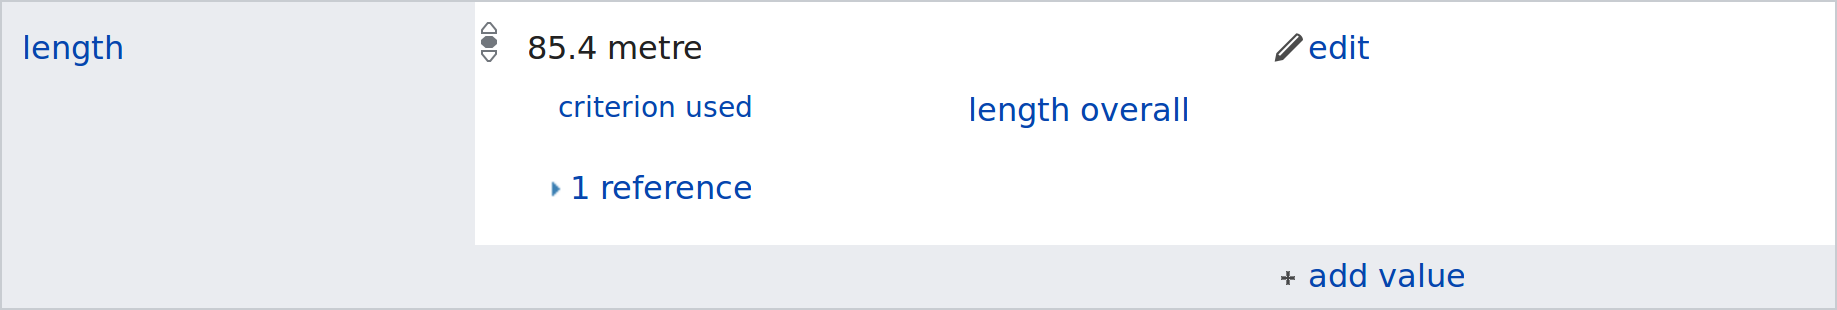
\includegraphics[width=\linewidth]{images/cutty_sark_length.png}
\caption{Statement with qualifier and reference about the length of the Cutty Sark}\label{fig_example}
\end{figure}
\end{example}

\section{Datalog}
Datalog is a logic query language. It is fully declarative and uses rules to derive additional knowledge from given facts. The most basic domain element in datalog is a \emph{constant}, which will be denoted as \emph{someConstant}. In the context of Wikidata, any item or property, e.g. \emph{Earth} (Q2) or \emph{head of government} (P6), could be represented as a constant. Relations in datalog are expressed using \emph{predicates} with a specified arity \(n\), written as predicate\([n]\). To stay close to Wikidata in our examples let us take the predicate triple\([3]\) as an example. This would be used to express the \emph{item}-\emph{property}-\emph{value} relation with each position representing one part of the triple.\\
Additionally, datalog also provides \emph{variables}, which will be capitalized like \(X\). The sets of predicates {\bf P}, constants {\bf C} and variables {\bf V} are mutually disjoint. Constants and variables are collectively known as \emph{terms} and are, together with predicates, used to form \emph{atoms}. An atom has the form predicate\((t_1, \ldots , t_n)\) with \(n\) as the arity of the predicate and \(t_1,\ldots,t_n\) terms.\\
Atoms are the building blocks of \emph{rules}, which are used to derive information in datalog. A rule is a premise that implies a conclusion, and both are conjunctions of atoms.
Let \(P_n\) denote  premise atoms and \(C_n\) the conclusion atoms. The variables used in one rule are divided into three mutually disjoint sets \(V_p\), \(V_c\), and \(V_r\) which are the variables occurring only in its premise atoms, only in its conclusion atoms, and occurring in both, respectively. The general from of an existential rule is (with \(k \in \mathbb{N}^+\), \(l \in \mathbb{N}\))
\begin{equation}
\forall V_p \forall V_r.(\exists V_c.C_1 \wedge \ldots \wedge C_k \leftarrow P_1 \wedge \ldots \wedge P_l)
\end{equation}

\(V_c\) are called existential variables. If \(V_c = \emptyset\) the rule is called a \emph{datalog rule} and if \(l = 0\) it is called a \emph{fact}. If a fact contains no variables but only constants it is a \emph{ground rule}. Since all \(V_p\) and \(V_r\) are  quantified, the preceding universal quantifiers \(\forall V_p \forall V_r\) will be omitted for the rules presented in this work.

Within the rule predicates we can differentiate between two different schemas: the \emph{extensional schema} and the \emph{intensional schema}, called EDB and IDB (extensional/intensional database). An EDB predicate may only occur in the premise of a rule, meaning it can never be derived. All predicates that appear in the conclusion at least once are IDB predicates.

\begin{example}
For the following example, taken from Wikidata, descriptive names will be used instead of the IDs to increase readability. The individual entities and properties are introduced with their ID beforehand so the example can be retraced. The species \emph{blue whale} (Q42196) has the \emph{parent taxon} (P171) \emph{balaenoptera} (Q133320), which in turn has the parent taxon \emph{rorqual} (Q232829). The predicates used are triple\_EDB\([3]\) as the input and isInTaxon\_IDB\([2]\), which will be derived. The basic facts are:
\[\text{triple\_EDB}(\text{blue whale}, \text{parent taxon}, \text{balaenoptera})\]
\[\text{triple\_EDB}(\text{balaenoptera}, \text{parent taxon}, \text{rorqual})\]
From this we can draw conclusions. The first step is to represent the already existing facts as IDB:
\[\text{isInTaxon\_IDB}(X, Y) \leftarrow \text{triple\_EDB}(X, \text{parent taxon}, Y)\]
Finally the transitive closure of this relation can be derived with
\[\text{isInTaxon\_IDB}(X, Y) \leftarrow \text{isInTaxon\_IDB}(X, Z) \wedge \text{isInTaxon\_IDB}(Z, Y)\]
\end{example}

\chapter{Property Constraints}\label{cha_property_constraints}

To improve the data quality, to help editors avoid common mistakes and to clarify the usage of properties, Wikidata allows constraints to be defined on properties. They are, however, not firm rules and exceptions can and should be made if necessary. A property constraint says something about the way a property may or may not be used. This can mean simple restrictions on the statement a property is part of, e.g. that only certain values are allowed, or more complex requirements on connected parts of the data, e.g. that the value of a statement with this property should have certain statements. In Table \ref{tab_property_constraints} you can find the existing property constraints as of September 2018. Afterwards the constraints will be explained in detail and their modelling given. For constraint that cannot be modelled, reasoning for this assessment is included.

To apply a constraint to a property, a statement <property> <P2302> <constraint> is added to the properties item page, where <property> is the property that should be constrained, <P2302> (property constraint) denotes that the property has a constraint and <constraint> is the specific constraint. Note that a constrained statement means a statement whose predicate is a property that has a specific constraint. A simple example for this would be \emph{distinct values} (Q21502410) stating that values of the property must be unique across all constrained statements. For this case no additional information regarding the constraint is necessary and violation could be found by surveying all constrained statements and comparing their values.\\
Constraints can be further specified by using qualifiers on the constraint statement. These qualifiers are either optional or mandatory and may be applied once or multiple times. For example, the \emph{none of} constraint (Q52558054) states that values for the specific property may not be in a given set of disallowed values. This set is specified using qualifiers with property \emph{item of} (P2305), which list all the disallowed values. At least one such qualifier must be present for the statement.\\
More complex dependencies are also possible. A constraint can depend on all constrained statements of a specific item (\emph{single value} constraint [Q19474404]), on all statements of the item specified as the value of a constrained statement (\emph{value requires statement} constraint [Q21510864]) or on all statements using the subclassOf-predicate (\emph{type} constraint [Q21503250]).

Table \ref{tab_property_constraints} shows all constraints that are used as of September 2018. It is roughly sorted by how difficult it is to model the given constraint using logical rules, based on the required expressive features and pre-processing. These required features are conditions that cannot natively be expressed in datalog and would require some kind of pre-processing of the dataset. Four constraints do not need any pre-processing except for loading the data into datalog as ground rules. Six can be solved if constant inequality is defined. This can be easily solved with brute force but will be improved in Section \ref{sec_inequality}. A further seven require negation of a specific fact which can be achieved with reasonable effort. The last ten are not deemed translatable because they require a feature that cannot be reasonably emulated in datalog. The feature mostly needed is a general form of negation that would allow to test for the non-existence of a derived fact. Other features needed for these constraints are regular expressions, which could theoretically be translated but would require large amounts of pre-processing, value comparison, and finally web requests to test if a link is valid.

\begin{table}[H]
\caption{property constraints}\label{tab_property_constraints}
\begin{tabularx}{\textheight}{rlll}
\makecell{\# constrained\\ properties} & Identifier & Name & Required Features \\
\hline
1410 & Q53869507 & Scope &  \\
781 & Q21502838 & Conflicts with &  \\
27 & Q52004125 & Allowed entity types &  \\
17 & Q52558054 & None of &  \\
\hline
2843 & Q21502410 & Distinct value & Inequality \\
343 & Q21514353 & Allowed units & Inequality \\
303 & Q21510851 & Allowed qualifiers & Inequality \\
116 & Q21510859 & One of & Inequality \\
3 & Q52060874 & Single best value & Inequality \\
1 & Q52712340 & One-of qualifier value & Inequality \\
\hline
4265 & Q21503247 & Item requires statement & Negation (statement non-existence) \\
244 & Q21510864 & Value requires statement & Negation (statement non-existence) \\
119 & Q21510855 & Inverse & Negation (statement non-existence) \\
33 & Q21510862 & Symmetric & Negation (statement non-existence) \\
13 & Q21510857 & Multi-value & Negation, Count (up to two) \\
2909 & Q19474404 & Single value & Inequality, Negation (qualifier non-existence) \\
203 & Q21510856 & Mandatory qualifier & Negation (qualifier non-existence) \\
\hline
2613 & Q21503250 & Type & Negation (derived fact negation) \\
707 & Q21510865 & Value type & Negation (derived fact negation) \\
3021 & Q21502404 & Format & Regular expressions \\
188 & Q21510860 & Range & Value comparison \\
106 & Q52848401 & Integer & Regular expressions \\
65 & Q51723761 & No bounds & Negation \\
53 & Q21510852 & Commons link & Web request \\
10 & Q54554025 & Citation needed & Negation \\
6 & Q21510854 & Difference within range & Value comparison \\
1 & Q25796498 & Contemporary constraint & Negation \\
\end{tabularx}
\end{table}

\section{Rules}
Table \ref{tab_property_constraints} shows that most constraints cannot be modelled without at least some amount of preprocessing. Only \emph{scope}, \emph{conflicts with}, \emph{allowed entity types} and \emph{none of} can be modelled directly. This is due to the fact that \emph{conflicts with} and \emph{none of} exclude a limited and specified set of statements from validity and these cases can thus be directly taken as violations. \emph{scope} and \emph{allowed entity types} work very similar, since there are only three respectively two possible values and violations are simply the options that have not been allowed. The rules for these constraints are described in Section \ref{sec_simple_constraints}.\\

A problem that occurs multiple times is the need to determine inequality between constants. \emph{distinct value}, \emph{allowed units}, \emph{allowed qualifiers}, \emph{one of}, \emph{single best value} and \emph{one-of qualifier value} each require a rule to determine if a value, unit or property is not equal to another. To this end a certain amount of preprocessing is necessary, most notably the extraction of all constant pairs whose inequality has to be determined for finding the violations. To avoid putting and undue amount of processing outside of datalog this extraction will not check more than that the constant is in the right position relative to the constrained statement, e.g., all values on statements constrained by \emph{distinct value} or all qualifiers on statements constrained by \emph{allowed qualifiers}. From this set inequality will be generated, different versions of which will be introduced in Section \ref{sec_inequality} and evaluated with regards to their performance in Section \ref{sec_inequality_evaluation}.\\

Negation as a general problem cannot be solved in datalog. One could pre-process every necessary fact to be negated and add this to the ground facts, but this is not the purpose of this work. However, not all constraints require a general negation. \emph{item requires statement}, \emph{value requires statement}, \emph{inverse }and \emph{symmetric} are all violated if a statement does not exist on a specific item. This problem can be solved with limited amounts of preprocessing by leveraging a preprocessed statement order per item and 'iterating' through the statements until the required conditions are met.\\
A similar approach can be taken to find items with exactly one statement matching certain criteria, required for 	\emph{multi-value}. The idea is to ask the question if a second statement exists, then evaluating it as above. Both methods will be explained in Section \ref{sec_statement_non-existence}.

\subsection{Representation of Wikidata as Facts}\label{subsec_representation}
To represent the content of Wikidata as facts the following predicates are introduced:
\begin{table}[H]
\caption{EDB predicates}\label{tab_predicates}
\begin{tabular}{llp{8.5cm}}
Predicate & Positions & Description \\
\hline
statement\_EDB & \makecell{statementID \\ entityID \\ propertyID \\ value (entityID or string)} & represents basic statements \\
\hline
qualifier\_EDB & \makecell{statementID \\ propertyID \\ value} & represents qualifiers on statements \\
\hline
reference\_EDB & \makecell{statementID \\ reference hash \\ propertyID \\ value} & represents references on statements; reference hash groups the property-value pairs belonging to one reference \\
\hline
item\_EDB & entityID & marks an entity as an item \\
property\_EDB & entityID & marks an entity as a property \\
\hline
unit\_EDB & \makecell{value \\ unitID} & denotes which unit a value has \\
\hline
rank\_EDB & \makecell{statementID \\ rank} & denotes the rank a statement has
\end{tabular}
\end{table}

\subsection{Terminology}
\begin{table}[H]
\caption{abbreviations}\label{tab_abbreviations}
\begin{tabular}{ll}
Shorthand & Description \\
\hline
constrained statement & statement with the constrained property as predicate \\
constrained qualifier & qualifier with the constrained property as predicate \\
constrained reference & reference with the constrained property as predicate \\
constrained entity & entity with a constrained statement \\
entity statement & statement on the same entity of a constrained statement \\
value statement & statement on the value of a constrained statement
\end{tabular}
\end{table}

\subsection{Task}\label{subsec_task}
Each property constraint will be modelled and evaluated as one set of rules per property per constraint, meaning each violating statement will be of a form similar to
\begin{align*}
&\text{violation\_statement}(S, E, \text{propertyConstant}, V) &\leftarrow \text{atoms determining the violation} \\
&\text{violation\_qualifier}(S, \text{propertyConstant}, V) &\leftarrow \text{atoms determining the violation} \\
&\text{violation\_reference}(S, H, \text{propertyConstant}, V) &\leftarrow \text{atoms determining the violation}
\end{align*}
where propertyConstant denotes the constrained property. The variables \(S\), \(I\), \(V\), and \(H\) are used for statement ID, entity ID, value and reference hash, respectively.

The task for each constraint is thus: Given the constraint and a constrained property, potentially with qualifiers, which rule finds all violations of the rule in a given set of triples, qualifiers and references if applicable? The given rule set should return all violations if queries with the following atoms:
\begin{align*}
&\text{violation\_statement}(S, E, P, V) \\
&\text{violation\_qualifier}(S, P, V) \\
&\text{violation\_reference}(S, H, P, V)
\end{align*}

\chapter{Wikidata constraints explained}\label{cha_wikidata_constraints_explained}
This Section will explain all interesting, meaning translatable or partially translatable, currently used property constraints on Wikidata. They will be presented roughly in descending order of the number of properties with this constraint, although constraints with similar function will be explained directly after one another. Additionally, all constraints that were considered untranslatable are listed at the and, each with a short explanation as to why they were placed in that group.

The constraints are described based on the Wikidata Property constraints portal\cite{constraintsPortal}, which links to a help page for every constraint. These help pages describe the constraint, list the possible or required qualifiers and show the intended usage with an example. In some cases the documentation was unclear and inquiries had to be made on the discussion pages of their respective constraints.

Every Section describing a constraint will consist of two subsections: the constraint explanation and the rules.

{\bf Constraint:} This subsection starts with a table showing basic properties of the constraint. These include the required data, relevant qualifiers, and possible violations of the constraint. The required data states which part of the data in relation to the constrained statement are restricted or need to exist. The qualifiers list their cardinality, meaning if they are required and if they may be used multiple times, and a short description. The violations list the conflicting (part of a) statement in relation to the constrained statement. The first constraint, \emph{property scope}, will be used as an example to explain the table in detail.

{\bf Rules:} Most constraints require more data than just the statements, qualifiers and references. This can include additional data from Wikidata to be provided as facts using the introduced predicates (see Table \ref{tab_predicates}), inequalities to be established as a pre-processing step (see Section \ref{sec_inequality}) or preparations to determine specific kinds of negation (see Section \ref{sec_statement_non-existence}). Afterwards, the rules necessary to determine violations are described.

\section{Simple Constraints}\label{sec_simple_constraints}
This Section contains constraints that do not require any additional features and can be translated into rules directly based on the facts introduced from Wikidata.

\subsection{Scope (Q53869507)}
\paragraph{Constraint}
The \emph{property scope} constraint specifies if a property may be used as predicate in a statement, qualifier or reference.
\begin{table}[H]
\caption{property scope constraint (Q53869507)}
\begin{tabularx}{\textwidth}{ ll X}
\hline
Required data & constrained statement, qualifier and reference \\
\hline
Qualifiers & \makecell{\emph{property scope} (P5314) -- 1..3 \\ must be \emph{as main value} (Q54828448), \emph{as qualifier} (Q54828449) \\ or \emph{as reference} (Q54828450) \\ specifies allowed use in statements, qualifiers or references} \\
\hline
Violation & constrained property in a position that is not allowed \\
\hline
\end{tabularx}
\end{table}

The required data specifies which data, in relation to the constrained statement, needs to be evaluated to conclude if the constraint was violated. The used abbreviations are listed in Table \ref{tab_abbreviations}. In this case this is simply each statement, qualifier or reference whose predicate is the constrained property.\\
The \emph{property scope} constraint requires the scope, meaning statement, qualifier or reference, to be set via qualifier \emph{property scope} (P5314). The cardinality is 1..3 because it is mandatory and has only three possible values.\\
It is violated if a statement, qualifier or reference has a predicate with the \emph{property scope} constraint that does not allow this scope.\\

\begin{example}
The \emph{reference URL} (P854) property is restricted to the \emph{property scope} (P5314) \emph{as reference} (Q54828450), because it is to be used to mark a URL that substantiates a statement.
\end{example}

\paragraph{Rules}
The property scope constraint requires no context information to be violated; the triple, qualifier, or reference with the constrained property is enough. This means violations can be found using these rules:
\begin{align*}
\text{violation\_statement}(S, I, \text{propertyConstant}, V) &\leftarrow \text{statement\_EDB}(S, I, \text{propertyConstant}, V)\\
\text{violation\_qualifier}(S, \text{propertyConstant}, V) &\leftarrow \text{qualifier\_EDB}(S, \text{propertyConstant}, V)\\
\text{violation\_reference}(S, \text{propertyConstant}, V) &\leftarrow \text{reference\_EDB}(S, H, \text{propertyConstant}, V)
\end{align*}
Which of these rules need to be used depends on the values of the \emph{property scope} qualifier. If a concrete constrained on a property does not have \emph{as main value} as a value of the qualifier, the first rule is used. The case for \emph{as qualifier} and \emph{as reference} is analogue with the second and third rule, respectively.

\subsection{Conflicts with (Q21502838)}
\paragraph{Constraint}
The \emph{conflicts with} constraint forbids statements on constrained entities whose predicate is a specified \emph{conflicting property}. If \emph{conflicting values} have been specified as well, the constraint is weakened and only violated by statements if in addition to the predicate being a \emph{conflicting property}, the object is one of the \emph{conflicting values}.
\begin{table}[H]
\caption{Conflicts-with constraint (Q21502838)}
\begin{tabularx}{\textwidth}{ ll X}
\hline
Required data & entity statements \\
\hline
Qualifiers & \makecell{\emph{conflicting property} (P2306) -- 1 \\ property that may not be predicate of entity statements \\
\emph{conflicting values} (P2305) -- 0..* \\ values that may not be objects of entity statements with the \emph{conflicting property}} \\
\hline
Violation & \makecell{entity statement with the conflicting property \\ entity statement with the conflicting property and one of the conflicting values} \\
\hline
\end{tabularx}
\end{table}

\begin{example}
The \emph{author} (P50) constraint has (among others) the \emph{conflicting property} (P2306) \emph{instance of} (P31) with the \emph{conflicting value} (P2305) \emph{Wikimedia disambiguation page} (Q4167410). It is set because editors might easily confuse a work of art with a specific title, e.g., \emph{Tempest} (Q86440) by \emph{author} \emph{William Shakespear} (Q692) with the Wikimedia disambiguation page \emph{Tempest} (Q1589529).
\end{example}

\paragraph{Rules}
The conflicts-with constraint is violated if another statement on the same item either has a conflicting property or a conflicting property and a conflicting value depending on specified qualifiers. It depends on a conjunction (\(O\) denoting another statement ID, \(C\) another value) and a violation for a conflicts-with constraint is thus either
\begin{equation*}
\begin{split}
\text{violation\_statement}&(S, I, \text{propertyConstant}, V) \leftarrow\\
&\text{statement\_EDB}(S, I, \text{propertyConstant}, V) \wedge{}\\
&\text{statement\_EDB}(O, I, \text{conflictingPropertyConstant}, C)
\end{split}
\end{equation*}
for constraints with no conflicting values specified or one
\begin{equation*}
\begin{split}
\text{violation\_statement}&(S, I, \text{propertyConstant}, V) \leftarrow\\
&\text{statement\_EDB}(S, I, \text{propertyConstant}, V) \wedge{}\\
&\text{statement\_EDB}(O, I, \text{conflictingPropertyConstant}, \text{conflictingValueConstant})
\end{split}
\end{equation*}
for each conflicting value if specified.\\

\subsection{Allowed entity types (Q52004125)}
\paragraph{Constraint}
The \emph{allowed entity types} constraint limits if a property may be used in a statement whose subject is an item, a property or a lexeme, although as of September 2018 lexemes are not deployed.

\begin{table}[H]
\caption{Allowed entity types constraint (Q52004125)}
\begin{tabularx}{\textwidth}{ ll X}
\hline
Required data & constrained statements and entity types\\
\hline
Qualifiers & \makecell{allowed entity type (P2305) -- 1..3 \\ must be \emph{Wikibase item} (Q29934200), \emph{Wikibase property} (Q29934218) \\ or lexeme (Q51885771); \\ specifies the entity type the property may be used on} \\
\hline
Violation & \makecell{constrained statement on an entity of a type unequal to all allowed types} \\
\hline
\end{tabularx}
\end{table}

Since there are only three options (and only two in use), violations can be found without inequality by finding the statement\_EDB with the constrained property whose subject is of the type that is not allowed, meaning either \emph{Wikibase item} or \emph{Wikibase property}.

\begin{example}
The \emph{property constraint} (P2302) property has the \emph{allowed entity type} (P2305) \emph{Wikibase property} (Q29934218) because non-properties cannot be subject to a property constraint.
\end{example}

\paragraph{Rules}
The allowed entity types constraint is violated by a statement with the wrong entity type.  Constraints regarding the lexeme entity type can be ignored since they are currently not used. The Violations depend on a simple conjunction:
\begin{equation*}
\begin{split}
\text{violation\_statement}&(S, I, \text{propertyConstant}, V) \leftarrow \\
&\text{statement\_EDB}(S, I, \text{propertyConstant}, V) \wedge \text{item}(I)
\end{split}
\end{equation*}
\begin{equation*}
\begin{split}
\text{violation\_statement}&(S, I, \text{propertyConstant}, V) \leftarrow \\
&\text{statement\_EDB}(S, I, \text{propertyConstant}, V) \wedge \text{property}(I)
\end{split}
\end{equation*}
The first rule are created for all \emph{allowed entity type} constraints whose \emph{allowed entity type} does not contain \emph{Wikibase item}. The second rule works analogue for \emph{Wikibase property}.

\subsection{None of (Q52558054)}
\paragraph{Constraint}
The none of constraint restricts the values that the property may refer to by listing a set of values as forbidden.

\begin{table}[H]
\caption{None of constraint (Q52558054)}
\begin{tabularx}{\textwidth}{ ll X}
\hline
Required data & constrained statements, qualifiers and references \\
\hline
Qualifiers & \makecell{\emph{forbidden value} (P2305) -- 1..* \\ values that may not be object of a constraint statement, qualifier or reference} \\
\hline
Violation & \makecell{constrained statement, qualifier or reference with a forbidden value} \\
\hline
\end{tabularx}
\end{table}

\begin{example}
The \emph{license} (P31) property, denoting the license under which a work is released, has the \emph{forbidden value} (P2305) \emph{proprietary software} (Q218616), since it is often confused with \emph{proprietary license} (Q3238057).
\end{example}

\paragraph{Rules}
The none of constraint simply forbids certain values for properties, thus effectively prohibiting certain triples, qualifiers and references. The rules, depending on nothing but specific database entries, are
\begin{equation*}
\begin{split}
\text{violation\_statement}&(S, I, \text{propertyConstant}, \text{forbiddenValueConstant}) \leftarrow \\
&\text{statement\_EDB}(S, I, \text{propertyConstant}, \text{forbiddenValueConstant})
\end{split}
\end{equation*}
\begin{equation*}
\begin{split}
\text{violation\_qualifier}&(S, \text{propertyConstant}, \text{forbiddenValueConstant}) \leftarrow \\
&\text{qualifier\_EDB}(S, \text{propertyConstant}, \text{forbiddenValueConstant})
\end{split}
\end{equation*}
\begin{equation*}
\begin{split}
\text{violation\_reference}&(S, \text{propertyConstant}, \text{forbiddenValueConstant}) \leftarrow \\
&\text{reference\_EDB}(S, H, \text{propertyConstant}, \text{forbiddenValueConstant})
\end{split}
\end{equation*}
Given a specified constraint, each of the three rules is created once for each \emph{forbidden value}.

\section{Constraints using Inequality}\label{sec_constraints_using_inequality}
All translatable constraints except the four covered in the previous Section require inequality in some way or another. This means it is necessary to extract additional information during pre-processing, namely the constants for which inequality needs to be stated. Each constraint will list the possible unequal entities in relation to the constrained statement. Multiple ways of implementing inequality while keeping the number of rules small will be discussed. Afterwards all constraints that can be translated using inequality will be explained.

\subsection{Approaches}
In every approach it will be necessary to load some basic inequalities into the database. To this end the predicate unequal\_EDB\([2]\) is introduced. Since the goal is to keep the number of applications of this predicate small, an IDB predicate unequal\([2]\) has to be introduced. This leads to the rule
\begin{equation*}
\text{unequal}(X, Y) \leftarrow \text{unequal\_EDB}(X, Y)
\end{equation*}

Given a set of unequal constants \(U\), the task is to generate rules so that for all \( x, y \in U: x \ne y \Rightarrow \text{unequal}(x, y)\).

\subsubsection{Naive}\label{subsubsec_naive}
The naive approach would be to simply add all possible combinations:
\begin{equation*}
\text{for all } x, y \in U, x \ne y \text{ add } \text{unequal\_EDB}(x, y)
\end{equation*}
This can be easily improved using the inverse and adding the following rule:
\begin{equation}\label{equ_inverse}
\text{unequal}(X, Y) \leftarrow \text{unequal}(Y, X)
\end{equation}
Then it is sufficient to add each combination once. To achieve this assume an arbitrary total order \(<\) has been established on the set \(E\):
\begin{equation*}
\text{for all } x, y \in U, x < y \text{ add } \text{unequal\_EDB}(x, y)
\end{equation*}

\subsubsection{Encoding constant strings to establish inequality}\label{subsubsec_encoding}
One way of determining inequality would be to take advantage of the fact that inequality is established in a set of unequal constants \(U\), which can be represented as a string. The idea is to determine the set of characters used in \(U\), set these characters as unequal as outlined in Section \ref{subsubsec_encoding} and associate each unequal constant with their characters.\\

An unequal constant \(u \in U\) can be represented a string and be written as \(c_0 \ldots c_{l - 1}\) with \(l = len(u)\) being the length of the string. Denote the set \(C\) as the set of characters occurring in unequal strings. Then \(l_{\max} = \max\limits_{\forall u \in U}(len(u))\) is the length of the longest entity string that occurs in the given data.
Based on this a group of predicates letter\(_i\)\_EDB[8] is introduced where \(0 \equiv i \mod 7\), \(0 \leq i < l_{max} \). 

For each unequal constant string \(u = c_0 \ldots c_{l - 1}\) and \(0 \equiv i \mod 7, 0 \leq i < len(u)\) an atom using predicate letter\(_i\)\_EDB is created as 
\begin{equation*}
\text{letter}_i\text{\_EDB}(e, f(e, i), f(e, i+1), \ldots, f(e, i+6)
\end{equation*}where
\begin{equation*}
f(e, i) = 
\begin{cases}
      c_i & i < len(e) \\
      \text{none} & i \geq len(e)
\end{cases}
\end{equation*}

Now that inequality between all characters and the link between entities and their characters are introduced, the inequality between two entities can be derived by creating the following rules for all predicates letter\(_i\)\_EDB (with \text{letters} short for \(\text{letter}_i\text{\_EDB}(X, A_i, \ldots, A_{i+6}) \wedge\text{letter}_i\text{\_EDB}(Y, B_i, \ldots, B_{i+6})\), \(i \leq j < i + 7\)):
\begin{equation*}
\text{unequal}(X, Y) \leftarrow \text{letters} \wedge \text{unequal}(A_j, B_j)
\end{equation*}
Note that the facts fulfilling \(\text{unequal}(A_j, B_j)\) are created by using the approach outlined in Section \ref{subsubsec_naive} for the set of characters \(C\) in all unequal constants \(U\).	

\subsubsection{Demand-driven materialisation}\label{subsubsec_demand-driven_materialisation}
The approaches outlined above will always result in all inequalities between the members of \(U\) being materialised. However, the purpose of determining inequality is to assist in finding violations of specific constraints. This means that only some inequalities -- the ones that actually appear in the dataset -- have to be evaluated. The rules can then be limited by introducing a new predicate req\_inequality\([2]\) which will only be derived if a condition occurs in which the inequality must be evaluated.\\

To save space and avoid redundancy the following rules will not explicitly state the inequality requirement predicate. Instead, assume that for every premise of the form \(B_1 \wedge \ldots\wedge B_m \wedge I_1 \wedge I_n\) where \(B_1 .. B_m\) are arbitrary atoms, \(I_1 .. I_n\) are atoms of the form \(\text{unequal}(t_{n_1}, t_{n_2})\) with \(t_{n_1}, t_{n_2}\) terms and all variables amount \(t_{n_1}\) and \(t_{n_2}\) appear in at least one of \(B_1 \ldots B_m\), the rules 
\begin{equation*}
\text{req\_inequality}(t_{n_1}, t_{n_2})
 \leftarrow B_1 \wedge \ldots \wedge B_m
\end{equation*} for all \(n\) are introduced.\\

The rules outlined in Section \ref{subsubsec_encoding} are changed to utilise this new requirement.
\begin{equation*}
\text{unequal}(X, Y) \leftarrow \text{req\_inequality}	(X, Y) \wedge \text{letters} \wedge \text{unequal}(A_j, B_j)
\end{equation*}

\subsection{Distinct values (Q21502410)}\label{subsec_distinct_values}
\paragraph{Constraint}
The \emph{distinct values} constraint forbids the existence of two constrained statements with the same object.
\begin{table}[H]
\caption{distinct values constraint (Q21502410)}
\begin{tabularx}{\textwidth}{ ll X}
\hline
Required data & constrained statements \\
\hline
Violations & two constrained statements with same value \\
\hline
Rule features & inequality \\
\hline
\end{tabularx}
\end{table}
The constraint can be expanded to cover qualifiers and references as well by setting a \emph{constraint scope} (P4680) qualifier with the respective value. However, as of September 2018 there is no constraint making use of this.

\begin{example}
The \emph{ISBN-13} (P212) property has a \emph{distinct values} constraint since an ISBN is supposed to be a unique identifier for a book and should not be shared between two items.
\end{example}

\paragraph{Rules}
The \emph{distinct values} constraint requires two distinct constrained statements with the same value. 
Two constrained statements with the same value can be found via a simple conjunction of two statement\_EDB atoms with the propertyConstant as predicate and a variable \(V\) as value. Since this would mark every constrained statement as a violations because it can fulfil both atoms at the same time, inequality of the statement IDs \(S\) and \(O\) must be tested as well.
\begin{equation*}
\begin{split}
\text{violation\_statement}&(S, I, \text{propertyConstant}, V) \leftarrow \\
&\text{statement\_EDB}(S, I, \text{propertyConstant}, V) \wedge{} \\
&\text{statement\_EDB}(O, X, \text{propertyConstant}, V) \wedge{} \\
&\text{unequal}(S, O)
\end{split}
\end{equation*}
The rules for qualifiers and reference are analogue.

\subsection{Allowed units (Q21514353)}\label{subsec_3_allowed_units}
\paragraph{Constraint}
The \emph{allowed units} constraint specifies that the value of a constrained statement may only have a unit that is in a set of specific units.

\begin{table}[H]
\caption{Allowed units constraint (Q21514353)}
\begin{tabularx}{\textwidth}{ ll X}
\hline
Required data & constrained statements \\
\hline
Qualifiers & \makecell{\emph{allowed unit} (P2305) -- 1..* \\ units that are allowed on values of constrained statements (\emph{none} for dimensionless units)} \\
\hline
Violation & \makecell{constrained statement with a unit unequal to all allowed units} \\
\hline
Rule features & inequality \\
\hline
\end{tabularx}
\end{table}

By setting the \emph{constraint scope} (P4680) qualifier on the constraint it can be limited to only affect a subset of statement, qualifier, and reference. As of September 2018 this is not done on any constraint.

\begin{example}
The \emph{length} (P2043) property has (among others) the \emph{allowed unit} (P2305) \emph{metre} (Q11573). This helps avoid confusing it for \emph{duration} (P2047), which denotes the length of time of an event.
\end{example}

\paragraph{Rules}
To handle this constraint inequality between all units need to be established. Then a violation can be identified by finding all statement\_EDB, qualifier\_EDB and reference\_EDB with the constrained property and a unit unequal to all allowed units.
The allowed units constraint needs to determine inequality between all allowed units and each unit on a constrained statement. To this end the units of a triple, qualifier or reference needs to be extracted during pre-processing and their inequality established. Quantities are rendered as string during pre-processing, specifying their value, bounds and unit.

To determine if a violation occurred, the unit of the constrained statement needs to be found. This is done via the unit-predicate as below
\begin{equation*}
\text{statement\_EDB}(S, I, \text{propertyConstant}, V) \wedge \text{unit\_EDB}(V, U)
\end{equation*}
with qualifiers and references treated analogue.

The complete rules require multiple unequal-atoms for all allowed units. Given a set \(A\) of constants, in this case allowed units, \(\text{unequal}(\{A\}, t)\) with an arbitrary term \(t\) is short for \(\bigwedge_{a \in A} \text{unequal}(a, t)\)

Violation are thus
\begin{equation*}
\begin{split}
\text{violation\_statement}&(S, I, \text{propertyConstant}, V) \leftarrow \\
&\text{statement\_EDB}(S, I, \text{propertyConstant}, V) \wedge{} \\
&\text{unit}(V, U) \wedge \text{unequal}(\{A\}, U)
\end{split}
\end{equation*}
\begin{equation*}
\begin{split}
\text{violation\_qualifier}&(S, I, \text{propertyConstant}, V) \leftarrow \\
&\text{qualifier\_EDB}(S, \text{propertyConstant}, V) \wedge{} \\
&\text{unit}(V, U) \wedge \text{unequal}(\{A\}, U)
\end{split}
\end{equation*}
\begin{equation*}
\begin{split}
\text{violation\_reference}&(S, I, \text{propertyConstant}, V) \leftarrow \\
&\text{reference\_EDB}(S, H, \text{propertyConstant}, V) \wedge{} \\
&\text{unit}(V, U) \wedge \text{unequal}(\{A\}, U)
\end{split}
\end{equation*}

\subsection{Allowed qualifiers (Q21510851)}
\paragraph{Constraint}
The \emph{allowed qualifiers} constraint specifies that only a limited set of properties may be used as predicates of qualifiers on a constrained statement.

\begin{table}[H]
\caption{Allowed qualifiers constraint (Q21510851)}
\begin{tabularx}{\textwidth}{ ll X}
\hline
Required data & qualifiers on constrained statements \\
\hline
Qualifiers & \makecell{\emph{allowed qualifier} (P2306) -- 1..* \\ properties that may appear in predicates of qualifiers on constrained statements} \\
\hline
Violation & \makecell{constrained statement with a qualifier unequal to all allowed qualifiers} \\
\hline
Rule features & inequality \\
\hline
\end{tabularx}
\end{table}

\begin{example}
The \emph{head of state} (P35) property has (among others) the \emph{allowed qualifiers} (P2306) \emph{start time} (P580) and \emph{end time} (P582) properties, used to describe the time frame the person held that office.
\end{example}

\paragraph{Rules}
To represent a violation of the \emph{allowed qualifiers} constraint in datalog inequality between all specified allowed qualifiers and the properties of qualifiers is required. The constraint is violated if a qualifier on a constrained statement exists that is unequal to all allowed qualifiers. The notation for set inequality as introduced in Section \ref{subsec_3_allowed_units} will be used. With \(A\) the set of allowed qualifiers the rule is:
\begin{equation*}
\begin{split}
\text{violation\_statement}&(S, I, \text{propertyConstant}, V) \leftarrow \\
&\text{statement\_EDB}(S, I, \text{propertyConstant}, V) \wedge{} \\
&\text{qualifier\_EDB}(S, Q, O) \wedge \text{unequal}(\{A\}, Q)
\end{split}
\end{equation*}

\subsection{One-of (Q21510859)}
\paragraph{Constraint}
The \emph{one-of} constraint limits the values of a constraint statement, qualifier or reference to a set of given values.

\begin{table}[H]
\caption{One-of constraint (Q21510859)}
\begin{tabularx}{\textwidth}{ ll X}
\hline
Required data & constrained statements, qualifiers and references \\
\hline
Qualifiers & \makecell{\emph{allowed values} (P2305) -- 1..* \\ values that may be used as objects of a constrained statement} \\
\hline
Violation & \makecell{constrained statement with a value unequal to all allowed values} \\
\hline
Rule features & inequality \\
\hline
\end{tabularx}
\end{table}

\begin{example}
The \emph{wheelchair accessibility} (P2846) property, which describes the accessibility of an location or event, has the three \emph{allowed values} (P2305) \emph{wheelchair accessible} (Q24192067), \emph{wheelchair accessible with help} (Q24192068), and \emph{wheelchair inaccessible} (Q24192069).
\end{example}

\paragraph{Rules}
The one-of constraint fits in the pattern established by the previous two constraints and disallows certain property-value combinations in statements, qualifiers and references. Inequality is established between all \emph{allowed values} and the values of statements, qualifiers and references, respectively. With \(A\) the set of allowed values the rules for triple, qualifier and reference are:
\begin{align*}
\text{violation\_statement}(S, I, \text{propertyConstant}, V) &\leftarrow \\
\text{statement\_EDB}(S, I, &\text{propertyConstant}, V) \wedge \text{unequal}(\{A\}, V) \\
\text{violation\_qualifier}(S, \text{propertyConstant}, V) &\leftarrow \\
\text{qualifier\_EDB}(S, &\text{propertyConstant}, V) \wedge \text{unequal}(\{A\}, V) \\
\text{violation\_reference}(S, \text{propertyConstant}, V) &\leftarrow \\
\text{reference\_EDB}(S, H, &\text{propertyConstant}, V) \wedge \text{unequal}(\{A\}, V)
\end{align*}

\subsection{One-of qualifier value (Q52712340)}
\paragraph{Constraint}
The \emph{one-of qualifier value} constraint restricts which \emph{qualifier values} may be used on a qualifier with a given \emph{qualifier property} on a constrained statement.

\begin{table}[H]
\caption{One-of qualifier value constraint (Q52712340)}
\begin{tabularx}{\textwidth}{ ll X}
\hline
Required data & constrained statements and their qualifiers \\
\hline
Qualifiers: & \makecell{\emph{qualifier property} (P2306) -- 1 \\ property that, if used as predicate, constrains a qualifier \\
\emph{qualifier values} (P2305) -- 1..* \\ values that are allowed for qualifiers on constrained statements \\ with the \emph{qualifier property} as predicate}\\
\hline
Violation & \makecell{constrained statement with a qualifier with the qualifier property \\ and a value unequal to all qualifier values} \\
\hline
Rule features & inequality \\
\hline
\end{tabularx}
\end{table}

\begin{example}
The \emph{flag bearer} (P3022) property, naming the person carrying a flag at a ceremony, has the \emph{qualifier property} (P2306) \emph{of} (P642) with the \emph{qualifier values} (P2305) \emph{opening ceremony} (Q3010369) and \emph{closing ceremony} (Q13454063).
\end{example}

\paragraph{Rules}
The one-of qualifier value constraint is violated if a constrained statement has a qualifier with a value unequal to all allowed values. Inequality needs to be established between all values of qualifiers and all allowed values. With the set of allowed Values \(A\) the rules are
\begin{equation*}
\begin{split}
\text{violation\_statement}&(S, I, \text{propertyConstant}, V) \leftarrow \\
&\text{statement\_EDB}(S, I, \text{propertyConstant}, V) \wedge{} \\
&\text{qualifier\_EDB}(S, \text{qualifierProperty}, O) \wedge \text{unequal}(\{A\}, O)
\end{split}
\end{equation*}

 \section{Constraints using Statement non-Existence}\label{sec_constraints_using_statement_non}
Several constraints are violated if specific statements do not exist in relation to constrained statements. It is not possible to simply negate said statements and pre-processing every required statement would defeat the purpose of implementing them in datalog. However, non-existence can be derived utilising the order of statements. Three predicates are introduced: first\([2]\), last\([2]\), and next\([2]\), which denote the first and last statement of an item and the following statement to another using their statement IDs.\\

If qualifier non-existence should be tested the predicates have to be adapted, since qualifiers do not have a unique identifier. To assign them a unique identity, statement ID, property and value have to be used. For this the predicates first\_qualifier\([3]\) and last\_qualifier\([3]\) taking the statement ID, the property and the value and next\_qualifier\([6]\) with ID, property and value for the current and next qualifier are introduced.\\

Using this pre-processed data, the approach is to apply a require-predicate to each statement or qualifier. This is require\([3]\) for statements, connecting the statement ID with the constrained property \(p\) and the required term \(t\) and require\([5]\) taking the statement ID, property, and value of a qualifier and linking this with \(p\) and \(t\).\\

For statements the pattern consists of two rules, both utilising the same conjunction \(c = C_1 \wedge \ldots \wedge C_m\) with atoms \(C_i\) depending on the constraint which is used to test if the statement does not fulfil the requirement. Then rule one
\begin{equation*}
\text{require}(S, p, t) \leftarrow \text{first}(S, I) \wedge c
\end{equation*}
states that the statement requires the condition and
\begin{equation*}
\text{require}(S, p, t) \leftarrow \text{next}(O, S) \wedge \text{require}(O, p, t) \wedge c
\end{equation*}
propagates this down the statement chain.

For qualifiers the rules are
\begin{equation*}
\text{require}(S, P, V, p, t) \leftarrow \text{first}(S, P, V) \wedge c
\end{equation*}
\begin{equation*}
\text{require}(S, P, V, p, t) \leftarrow \text{next}(O, X, C, S, P, V) \wedge \text{require}(O, X, C, p, t) \wedge c
\end{equation*}

If the last statement of an item or the last qualifier of a statement has require the violation occurred. In the following constraints only the conjunction \(c\) and adjustments to this pattern will be described. The require-propagation is regarded as given.

\subsection{Item requires statement (Q21503247)}\label{subsec_item_requires_statement}
\paragraph{Constraint}
The \emph{item requires statement} constraint requires an additional statement on an item with a statement using the constrained property. It can be even more restrictive by also requiring the value of said additional statement to be in a set of \emph{allowed values}.
\begin{table}[H]
\caption{item requires statement constraint (Q21503247)}\label{tab_item_requires_statements}
\begin{tabularx}{\textwidth}{ ll X}
\hline
Required data & item statements \\
\hline
Qualifiers & \makecell{\emph{required property} (P2306) -- 1 \\ property that must be predicate of an item statement \\
\emph{allowed value} (P2305) -- 0..* \\ value that must be object of the item statement} \\
\hline
Violation & \makecell{no item statement with required property \\ all item statements with required property have no allowed value} \\
\hline
Rule features & negation \\
\hline
\end{tabularx}
\end{table}

\begin{example}
The \emph{professorship} (P803) property requires an additional statement with the \emph{required property} (P2306) \emph{occupation} (P106) and the \emph{allowed value} (P2305) \emph{university teacher} (Q1622272).
\end{example}

\paragraph{Rules}
The \emph{item requires statement} constraint requires inequality between all properties of statements and the \emph{required property} as well as between all statement values and the \emph{allowed values}. The order of the item statements needs to be established. An item violates the constraint if it a) has a statement using constrained property as predicate, b1) has no statement using the \emph{required property} as predicate, or (if \emph{allowed values} are specified) b2) has only statement using the \emph{required property} as predicate that do not use one of the \emph{allowed values} as value. The required term \(t\) is the \emph{required property}. Without separators the conjunction is
\begin{equation*}
\begin{split}
c_1 = &\text{statement\_EDB}(Q, I, \text{propertyConstant}, X) \wedge{} \\
&\text{statement\_EDB}(S, I, P, V) \wedge \text{unequal}(\text{requiredPropertyConstant}, P)
\end{split}
\end{equation*} \(\)
If a set of \emph{allowed values} \(A\) has been specified, a second set of require-rules have to be introduced with
\begin{equation*}
\begin{split}
c_2 = &\text{statement\_EDB}(Q, I, \text{propertyConstant}, X) \wedge{} \\
&\text{statement\_EDB}(S, I, \text{requiredPropertyConstant}, V) \wedge \text{unequal}(\{A\}, V)
\end{split}
\end{equation*}
Note that the first set of rules is still required, since the preceding statements do not need to have the \emph{required property}. In both cases violations can be found with
\begin{equation*}
\begin{split}
\text{violation\_statement}&(S, I, \text{propertyConstant}, V) \leftarrow \\
&\text{statement\_EDB}(S, I, \text{propertyConstant}, V) \wedge{} \text{last}(O, I) \wedge{} \\
&\text{require}(O, \text{propertyConstant}, \text{requiredPropertyConstant})
\end{split}
\end{equation*}

\subsection{Value requires statement (Q21510864)}\label{subsec_value_requires_statement}
\paragraph{Constraint}
The \emph{value requires statement} constraint requires an additional statement on the value of constrained statement, possibly also using a specific value from the list of allowed values. Since the constraint works very similar to item requires statement (see \ref{subsec_item_requires_statement}) --- requiring a statement on the value of the constrained statement instead of on the item --- Table \ref{tab_item_requires_statements} is not repeated.

\begin{example}
The \emph{list of monuments} (P1456) property requires its value to have the \emph{required property} (P2306) \emph{is a list of} (P360).
\end{example}

\paragraph{Rules}
The \emph{value requires statement} constraint is syntactically very similar to the previous \emph{item requires statement} constraint. Instead of requiring a statement on the item of a constrained statement it requires it on the value. Inequality need to be computed between all properties and all values and the item statement order established. The conjunctions change in the first statement and are:
\begin{equation*}
\begin{split}
c_1 = &\text{statement\_EDB}(Q, R, \text{propertyConstant}, I) \wedge{} \\
&\text{statement\_EDB}(S, I, P, V) \wedge \text{unequal}(\text{requiredPropertyConstant}, P)
\end{split}
\end{equation*} \(\)
\begin{equation*}
\begin{split}
c_2 = &\text{statement\_EDB}(Q, R, \text{propertyConstant}, I) \wedge{} \\
&\text{statement\_EDB}(S, I, \text{requiredPropertyConstant}, V) \wedge \text{unequal}(\{A\}, V)
\end{split}
\end{equation*}
The final violation rule would then be:
\begin{equation*}
\begin{split}
\text{violation\_statement}&(S, I, \text{propertyConstant}, V) \leftarrow \\
&\text{statement\_EDB}(S, I, \text{propertyConstant}, V) \wedge{} \text{last}(O, V) \wedge{} \\
&\text{require}(O, \text{propertyConstant}, \text{requiredPropertyConstant})
\end{split}
\end{equation*}

\subsection{Inverse (Q21510855)}\label{subsec_2_inverse}
\paragraph{Constraint}
The \emph{inverse} constraint requires an additional statement on the value of a constrained statement with an \emph{inverse property} and the constrained item as value. It is very similar to \emph{value requires statement} (see \ref{subsec_value_requires_statement}), although it does not specify allowed values, since the required statement needs to have one specific value: the item of the constrained statement.

\begin{example}
The \emph{mother} (P25) property requires values to have a statement with the \emph{inverse property} (P2306) \emph{child} (P40) and the original item as value.
\end{example}

\paragraph{Rules}
The \emph{inverse} constraint can be modelled in almost the same way as the \emph{value requires statement} constraint. The only change is that instead of requiring inequality to all \emph{allowed values} in conjunction \(c_2\) the statement requires this constraint if its value is not the subject \(R\) of the original constrained statement, meaning \(t = R\). Inequalities have to be established between all properties and the \emph{inverse} property as well as all subjects and values of statements.
\begin{equation*}
\begin{split}
c_1 = &\text{statement\_EDB}(Q, R, \text{propertyConstant}, I) \wedge{} \\
&\text{statement\_EDB}(S, I, P, V) \wedge{} \\
&\text{unequal}(\text{inversePropertyConstant}, P)
\end{split}
\end{equation*}
\begin{equation*}
\begin{split}
c_2 = &\text{statement\_EDB}(Q, R, \text{propertyConstant}, I) \wedge{} \\
&\text{statement\_EDB}(S, I, \text{inversePropertyConstant}, V) \wedge{} \\
&\text{unequal}(R, V)
\end{split}
\end{equation*}
The final violation rule remains the same.

\subsection{Symmetric (Q21510862)}
The \emph{symmetric} constraint requires an additional statement on the value of a constrained statement with the constrained property and the constrained item as value. It is thus equal to an \emph{inverse} constraint (see \ref{subsec_2_inverse}) with the same property as constrained property and inverse property. It can be translated exactly as the inverse constraint if the inverse property where set to the same as the constrained property.

\begin{example}
The \emph{sibling} (P3373) property requires a statement on the value with the same property and the original item as the value.
\end{example}

\subsection{Multi-value (Q21510857)}
\paragraph{Constraint}
The \emph{multi-value} constraint specifies that the constrained property should appear in multiple statements of an item or none.

\begin{table}[H]
\caption{Multi-value constraint (Q21510857)}
\begin{tabularx}{\textwidth}{ ll X}
\hline
Required data & item statements \\
\hline
Violation & \makecell{constrained item with exactly one constrained statement} \\
\hline
Dependency & all item statements \\
\hline
Rule features & count \\
\hline
\end{tabularx}
\end{table}

\begin{example}
The \emph{cast member} (P161) property requires an item to have multiple statements using this property, since most plays or films have multiple cast members. This is an example for a constraint from which exception can and should be made and is only meant to point to possibly missing data.
\end{example}

\paragraph{Rules}
The \emph{multi-value} constraint requires a limited count of constrained statements. Alternatively, it could be said that if the item requires a second statement, the constraint is violated. Inequality is established between all properties of statements and the conjunction is:
\begin{equation*}
\begin{split}
c = &\text{statement\_EDB}(Q, I, \text{propertyConstant}, X) \wedge{} \\
&\text{statement\_EDB}(S, I, P, V) \wedge \text{unequal}(\text{propertyConstant}, P)
\end{split}
\end{equation*}
The predicate require\_second\([2]\) is introduced with the same meaning as require except that it will be applied after a required property has been found:
\begin{equation*}
\begin{split}
\text{require\_second}&(S, \text{propertyConstant}, \text{propertyConstant}) \leftarrow \\
&\text{next}(R, S) \wedge \text{statement\_EDB}(R, I, \text{propertyConstant}, C) \wedge{} \\
&\text{next}(Q, R) \wedge \text{require}(Q, \text{propertyConstant}, \text{propertyConstant})  \wedge c
\end{split}
\end{equation*}
\begin{equation*}
\begin{split}
\text{require\_second}&(S, \text{propertyConstant}, \text{propertyConstant}) \leftarrow \text{next}(R, S) \wedge{} \\
&\text{require\_second}(R, \text{propertyConstant}, \text{propertyConstant}) \wedge c
\end{split}
\end{equation*}
A violations would be any last statement requiring a second constrained statement.\\

\subsection{Single value (Q19474404)}\label{subsec_single_value}
\paragraph{Constraint}
The \emph{single value} constraint states that the constrained property may only be used once per item. A constrained statement marked with the single value constraint can have \emph{separators}, which define exceptions under specific circumstances.
\begin{table}[H]
\caption{single value constraint (Q19474404)}
\begin{tabularx}{\textwidth}{ ll X}
\hline
Required data & constrained statements and their qualifiers, constrained qualifiers and references \\
\hline
Qualifiers & \makecell{\emph{separator} (P4155) -- 0..* \\ qualifiers that, when used on constrained statements, can warrant an exception} \\
\hline
Violation & \makecell{two constrained statements with same item and value \\ (exception: statements with separators as qualifiers with different values)} \\
\hline
Rule features & inequality, partially negation \\
\hline
\end{tabularx}
\end{table}

If no separators are specified, two statements form a violation of this constraint if they a) belong to the same item, b) have the same constrained property, and c) have the same value.
If separators are specified, a violation as above can be ignored if the statements each have at least one qualifier with the same separator as predicate and different values or an unequal number of separator qualifiers.

\begin{example}
The \emph{capital} (P36) property should only have one single value per item. If conflicts exist, it is not a violation of this constraint if one of the values for the \emph{separators} (P4155) \emph{start time} (P580), \emph{point in time} (P585), \emph{end time} (P582), and \emph{determination method} (P459) are unequal.
\end{example}

\paragraph{Rules}
The single value constraint can be divided into two different cases, depending on if the set of separators \(S\) is empty or not. Pre-processing needs to extract all item statements and their qualifiers and establish inequality between all statement IDs and all qualifier values.

\subsubsection{No separators}\label{subsubsec_single_value_no_separators}
If the separator set is empty, the violation simply occurs if there are two constrained statements on the same item. 
\begin{equation}\label{eq_no_separators_triple}
\begin{split}
\text{violation\_statement}&(S, I, \text{propertyConstant}, V) \leftarrow \\
&\text{statement\_EDB}(S, I, \text{propertyConstant}, V) \wedge{} \\
&\text{statement\_EDB}(O, I, \text{propertyConstant}, X) \wedge{} \\
&\text{unequal}(S, O)
\end{split}
\end{equation}
For qualifiers and references there is no ID whose inequality could be checked. However, since the statement ID and the property of a possible conflict are always the same, inequality can be tested on the values.
\begin{equation*}
\begin{split}
\text{violation\_qualifier}&(S, \text{propertyConstant}, V) \leftarrow \\
&\text{qualifier\_EDB}(S, \text{propertyConstant}, V) \wedge{} \\
&\text{qualifier\_EDB}(S, \text{propertyConstant}, X) \wedge{} \\
&\text{unequal}(V, X)
\end{split}
\end{equation*}
\begin{equation*}
\begin{split}
\text{violation\_reference}&(S, H, \text{propertyConstant}, V) \leftarrow \\
&\text{reference\_EDB}(S, H, \text{propertyConstant}, V) \wedge{} \\
&\text{reference\_EDB}(S, J, \text{propertyConstant}, X) \wedge{} \\
&\text{unequal}(V, X)
\end{split}
\end{equation*}

\subsubsection{With separators}\label{subsubsec_single_value_with_separators}
To find all violations under \emph{separators} a number of things have to be considered. Only statements are eligible, since qualifiers cannot have further qualifier. The order of qualifiers on constrained statements needs to be provided as well since qualifier non-existence is relevant. The pattern needs to be applied for every \emph{separator}, meaning the conjunction is
\begin{equation*}
c = \text{statement\_EDB}(S, I, \text{propertyConstant}, C) \wedge \text{qualifier\_EDB}(S, P, V) \wedge \text{unequal}(P, \text{separatorConstant})
\end{equation*}
for each separator in \(S\).\\

With qualifier non-existence established the violation can be found. Two statements form a violation if they are distinct as per equation \ref{eq_no_separators_triple} and additionally fulfil the condition that all values of \emph{separator} qualifiers are equal or no such \emph{separator} qualifier exist. To determine this a number of rules have to be introduced which are based on two sets the \emph{separators} are split into: \(X\) contains the \emph{separators} that exist as qualifiers and \(Y\) the \emph{separators} that do not. The following rule is then created for every possible split of the \emph{separators} into two such sets. Note that \(\text{predicate}(\{X\})\) denotes \(\bigwedge_{x \in X} \text{predicate}(x)\) as introduced in Section \ref{subsec_3_allowed_units}.
\begin{equation*}
\begin{split}
\text{violation\_statement}&(S, I, \text{propertyConstant}, V) \leftarrow \\
&\text{statement\_EDB}(S, I, \text{propertyConstant}, V) \wedge{} \\
&\text{statement\_EDB}(O, I, \text{propertyConstant}, C) \wedge{} \\
&\text{unequal}(S, O) \wedge{} \\
&\text{has\_same}(S, O, \{X\}) \wedge{} \\
&\text{does\_not\_have}(S, \{Y\}) \wedge{} \\
&\text{does\_not\_have}(O, \{Y\})
\end{split}
\end{equation*}
The predicate does\_not\_have\([2]\) linking a statement ID to the separator it does not have via 
\begin{equation*}
\begin{split}
\text{does\_not\_have}(S, R) \leftarrow &\text{statement\_EDB}(S, I, \text{propertyConstant}, C) \wedge{} \\
&\text{last\_qualifier}(S, P, V) \wedge \text{require}(S, P, V, \text{propertyConstant}, R)
\end{split}
\end{equation*}
and the predicate has\_same[2] linking two statement IDs to the separator for which the values are the same via
\begin{equation*}
\begin{split}
\text{has\_same}(S, O, Q) \leftarrow &\text{statement\_EDB}(S, I, \text{propertyConstant}, C) \wedge{} \\
&\text{statement\_EDB}(O, I, \text{propertyConstant}, X) \wedge{} \\
&\text{qualifier\_EDB}(S, Q, V) \wedge \text{qualifier\_EDB}(O, Q, V)
\end{split}
\end{equation*}
are introduced for brevity.

\subsection{Mandatory qualifier (Q21510856)}
\paragraph{Constraint}
The \emph{mandatory qualifier} constraint requires that a constrained statement has a qualifier with a \emph{required property}.

\begin{table}[H]
\caption{Mandatory qualifier constraint (Q21510856)}
\begin{tabularx}{\textwidth}{ ll X}
\hline
Required data & constrained statements and their qualifiers \\
\hline
Qualifiers & \makecell{\emph{required property} (P2306) -- 1 \\ property that must appear as predicate of a qualifier on the constrained statement} \\
\hline
Violation & \makecell{constrained statement without a qualifier with the required property} \\
\hline
Rule features & negation \\
\hline
\end{tabularx}
\end{table}

\begin{example}
The \emph{head of state} (P35) property has the \emph{required property} (P2306) \emph{start time} (P580), meaning every \emph{head of state} must have assumed that position at some time.
\end{example}

\paragraph{Rules}
The \emph{mandatory qualifier} constraint needs to determine qualifier non-existence on constrained statements to find violations, which is similar to Section \ref{subsubsec_single_value_with_separators}. The qualifier order needs to be provided and inequality must be established between all qualifier properties. The conjunction for the require-pattern is:
\begin{equation*}
\begin{split}
c = &\text{statement\_EDB}(S, I, \text{propertyConstant}, C) \wedge{} \\
&\text{qualifier\_EDB}(S, P, V) \wedge \text{unequal}(P, \text{requiredPropertyConstant})
\end{split}
\end{equation*}
With the usual require-pattern for qualifiers and the does\_not\_have rule as introduced in Section \ref{subsubsec_single_value_with_separators} added for brevity the violations would be found with:
\begin{equation*}
\begin{split}
\text{violation\_statement}&(S, I, \text{propertyConstant}, V) \leftarrow \\
&\text{statement\_EDB}(S, I, \text{propertyConstant}, V) \wedge \\
&\text{does\_not\_have}(S, \text{requiredPropertyConstant})
\end{split}
\end{equation*}

\subsection{Single best value (Q52060874)}\label{subsec_single_best_value}
\paragraph{Constraint}
The \emph{single best value} constraint requires that only one constrained statement per item has the rank preferred.

\begin{table}[H]
\caption{Single best value constraint (Q52060874)}
\begin{tabularx}{\textwidth}{ ll X}
\hline
Required data & item statements and ranks \\
\hline
Qualifiers & \makecell{\emph{separator} (P4155) -- 0..* \\ qualifiers that, when used on constrained statements, can warrant an exception } \\
\hline
Violation & \makecell{items with two constrained statements with rank preferred \\ (exception: statements with separators as qualifiers with different values)} \\
\hline
Rule features & inequality, partially negation \\
\hline
\end{tabularx}
\end{table}

\begin{example}
The \emph{property proposal discussion} (P3254) property, denoting the URL of a web page where the creation of a Wikidata property was discussed should only have one best value. Since a discussion might have been moved to a different page at some point, the best value should be the page the discussion was last moved to.
\end{example}

\paragraph{Rules}
The \emph{single best value} constraint, like the \emph{single value} constraint (Section \ref{subsec_3_single_value}), differentiates between the set of \emph{separators} \(S\) being empty or not. Since the constraint depends on the rank of statements this needs to be provided. Qualifiers and references are not affected since they do not have ranks. For this constraint all inequality needs to be established between the statement IDs and the qualifier values as well as the order of the qualifiers given.\\

\subsubsection{No separators}
If the \emph{separator} set is empty, the violation simply occurs if there are two constrained statements on the same item with the preferred rank. Thus the rule \eqref{eq_no_separators_triple} is expanded to
\begin{equation*}
\begin{split}
\text{violation\_statement}&(S, I, \text{propertyConstant}, V) \leftarrow \\
&\text{statement\_EDB}(S, I, \text{propertyConstant}, V) \wedge{} \\
&\text{rank\_EDB}(S, \text{preferredRankConstant}) \wedge{} \\
&\text{statement\_EDB}(O, I, \text{propertyConstant}, X) \wedge{} \\
&\text{rank\_EDB}(O, \text{preferredRankConstant}) \wedge{} \\
&\text{unequal}(S, O)
\end{split}
\end{equation*}

\subsubsection{With separators}
As in the case above, the qualifier non-existence and violation rules are very similar to the \emph{single value} constraint. The only change is the addition of the rank requirements as shown below.
\begin{equation*}
\begin{split}
\text{violation\_statement}&(S, I, \text{propertyConstant}, V) \leftarrow \\
&\text{statement\_EDB}(S, I, \text{propertyConstant}, V) \wedge{} \\
&\text{rank\_EDB}(S, \text{preferredRankConstant}) \wedge{} \\
&\text{statement\_EDB}(O, I, \text{propertyConstant}, W) \wedge{} \\
&\text{rank\_EDB}(O, \text{preferredRankConstant}) \wedge{} \\
&\text{unequal}(S, O) \wedge{} \\
&\text{has\_same}(S, O, \{X\}) \wedge{} \\
&\text{does\_not\_have}(S, \{Y\}) \wedge{} \\
&\text{does\_not\_have}(O, \{Y\})
\end{split}
\end{equation*}

\section{Reasoning for unconsidered constraints}
Multiple constraints have not been described above for different reasons. The most prominent of these is the \emph{format} constraint (Q21502404) which specifies a regular expressions the values of the constrained property must adhere to. Evaluating these expressions would be theoretically possible but \\
\begin{enumerate}[a)]
\item primarily results in a large amount of preprocessing and
\item does not solve the question of negation, since violations would be values that do not conform to their required regular expression
\end{enumerate}

The two type constraints \emph{type} (Q21503250) and \emph{value type} (Q21510865) require an entity to have a certain type. This is defined transitively via the properties \emph{instance of} (P31) and \emph{subclass of} (P279), which have to form a statement chain to the entity given as the type. Evaluating these constraints would require pre-processing to compute all types of an entity transitively, add these as statements to the data and establish their order to allow testing for the non-existence of a type. Since the constraint could easily be checked when computing the types of an entity (is the required type in the types it has), this does not make sense in datalog.

The \emph{integer} constraint (Q52848401), which requires values of a constrained property be integers (notably a quantity without decimal places), could easily be seen as a specific format constraint. While precomputing if a value is an integer or not could be done, it would mean that no actually relevant rules would be needed for the evaluation in datalog.

Another problem that could not be sensibly solved is the comparison of values, needed for \emph{range} (Q21510860), \emph{difference within range} (Q21510854) and \emph{contemporary} constraint (Q25796498). \emph{Range} restricts the values of a constrained property within a certain range, \emph{difference within range} specifies that the values of two item statements should be within a certain range and \emph{contemporary} constraint specifies that subject and object of a constrained statement have to have coexisted at some point in time. While it would be possible to extract all values that might need to be compared and precompute the comparison, it would make most of the work precomputing and leave little to be done in datalog.

\emph{Citation needed} constraint (Q54554025), stating that constraint statements must have one or more references, requires a negation that cannot be concluded except by explicitly precomputing it, which makes the evaluation unnecessary. \\
A similar situation is the \emph{no bounds} constraint (Q51723761), which requires that quantity values have neither upper nor lower bound. While it would be possible to precompute if a statement has no upper or lower bound, this would shift basically all evaluation logic into precomputing.

And finally \emph{commons link} constraint (Q21510852) requires that values for a property should be valid links to to Wikimedia Commons. This validity cannot be tested from within datalog since there is no way to query the web for information.

\chapter{Evaluation}\label{cha_evaluation}

To evaluate the rules described in Chapter \ref{cha_wikidata_constraints_explained} they have been implemented for VLog4J \cite{vlog4j}. VLog4J is a java library base on VLog \cite{vlog}, a Datalog engine utilising a column-based memory layout to allow processing of large datasets on commodity hardware. It was first published in 2016\cite{UJK2016} but has been actively developed since then.

The entire content of Wikidata is available in several formats: the aforementioned RDF, JSON and XML. To evaluate the violations, Wikidata needs to be provided in form of atoms as described in 
Section \ref{subsec_representation}. For this purpose the Wikidata Toolkit (WDTK)\cite{wdtk} was used. It provides an iterator over the JSON dumps, allowing the processing of all entities in Wikidata.

The evaluation aims to document how suitable Datalog and VLog in particular are to extract violations from Wikidata. The performance impact of the additionally introduced features, inequality (Section \ref{sec_constraints_using_inequality}) and statement non-existence (Section \ref{sec_constraints_using_statement_non}) is evaluated.

\section{Software structure}
The evaluation software\cite{wcd} was written in Java and utilises WDTK and VLog4J to evaluate the violation rules on the content of Wikidata. Figure \ref{fig_pipeline} illustrates the steps undertaken to evaluate the constraints.

At the beginning the content of the Wikidata JSON-Dump, read via WDKT, is transformed into facts readable by VLog4J. These take the form of comma-separated value files which created for each predicate in Section \ref{subsec_representation}, denoted as "Facts" in the diagram.

Based on this set the Inequaliy Helper creates all files necessary to established inequality as described in Section \ref{sec_constraints_using_inequality}, based on which approach was chosen.

The rules determining violations are created by the Constraint Checker, which uses the Wikidata Query Service\footnote{\url{query.wikidata.org}} to fetch the current constraint configurations. Based on these configurations the rules are created as described in Chapter \ref{cha_wikidata_constraints_explained}.

Computing all violations based on the provided (inequality)-facts and violations rules is done per constraint. All facts pertaining to the constraint as well as the rules are loaded into VLog, which creates and in-memory database from the provided .csv-files. Once this is done, the reasoning engine materializes all possible facts. Afterwards, all violations are extracted by querying the database for the queries described in Section \ref{subsec_task}.

\begin{figure}
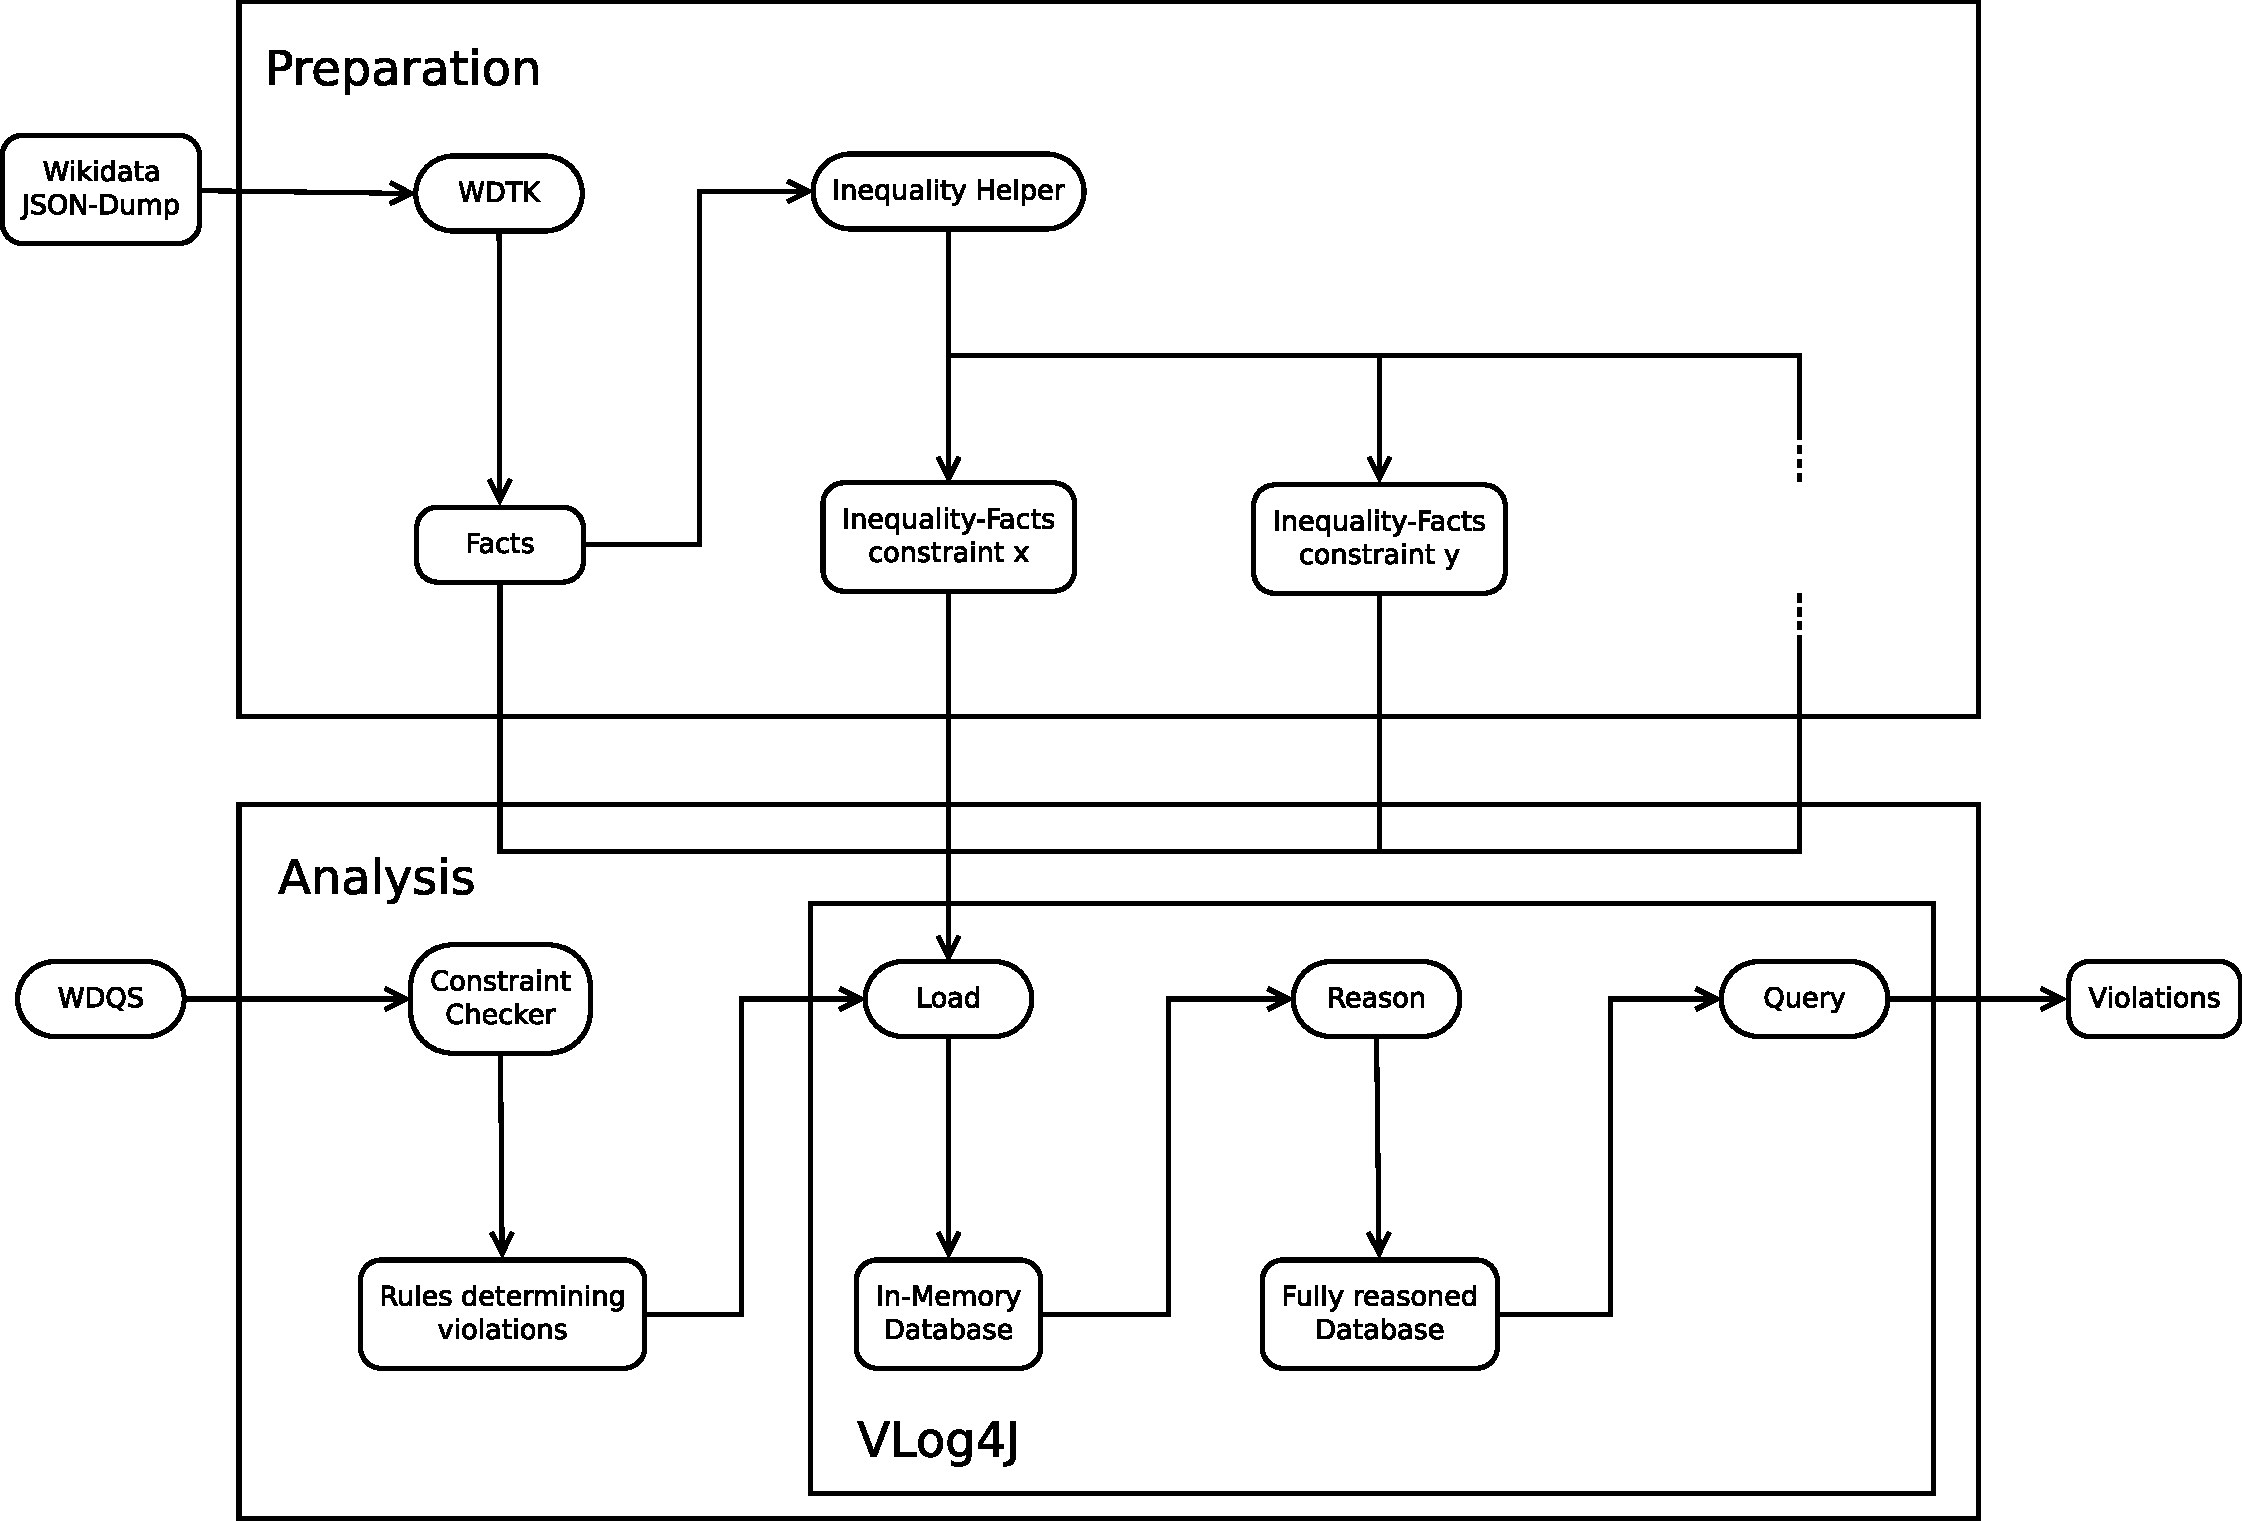
\includegraphics[width=\linewidth]{images/Pipeline.pdf}
\caption{Evaluation pipeline}\label{fig_pipeline}
\end{figure}

\section{Results}\label{sec_results}

The experiments where carried out on a server with a 3.50GHz Intel Xeon CPU, 1 TB SSD and 32 GB assigned RAM running Debian 4.9. Multiple sets of sizes ranging from one thousand to one million entities where extracted from the Wikidata JSON-Dump and all constraints evaluated against them.

\subsection{Statistics}
Several statistics about the executed runs are reported.

{\bf Runtime materialization} is the time taken by the VLog engine to compute all facts that can be derived from the given input.

{\bf Additional Derivations} counts how many new facts were created during materialization, excluding the violations themselves. 

{\bf Total Rules} states how many rules where created to establish the violations. They are split into two subfields: {\bf Demand rules}, which are additional rules created to satisfy the requirements outlined in Section \ref{subsubsec_demand-driven_materialisation}, and {\bf Base Rules}, which are the rules created without accounting for the demand-driven scheme.

\subsection{Overview}

Because of a bug in VLog\footnote{\url{https://github.com/knowsys/vlog4j/issues/43}}, the largest dataset that could be completely evaluated contained 100,000 entities. With datasets of larger size, more than half of the constraints were affected by this bug, meaning the analysis could not be conducted. All further statistics describe the results on the 100,000 entity set unless specifically noted otherwise. Since inequality could only be computed in demanded mode (see Section  \ref{sec_inequality_evaluation}), all statistics will show the results attained in this mode.

Most constraints could be evaluated in under a minute. The exceptions are \emph{distinct values} (1.22 hours), \emph{item requires statement} (2.38 hours) and \emph{single value} (4.22 hours). In parts this is expected behaviour, since these three constraints are applied to an order of magnitude more properties than all other properties with the exception of \emph{scope}, which is described in very simple rules. However, also seen in Figure \ref{fig_runtime}, the runtimes of these three constraints are multiple orders of magnitude higher than those of other constraints. The following Sections will thus focus on the comparison of these three constraints to identify bottlenecks and reasons for this huge difference in performance. They will be marked with a border in every figure.

\begin{figure}
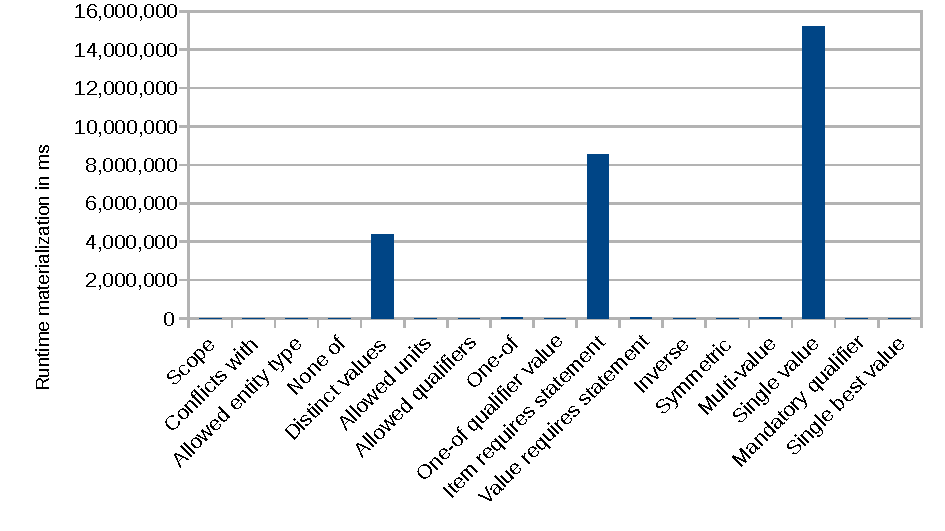
\includegraphics[width=\linewidth]{images/runtime100,000.pdf}
\caption{Runtime materialization for 100,000 entities}\label{fig_runtime}
\end{figure}

\begin{figure}
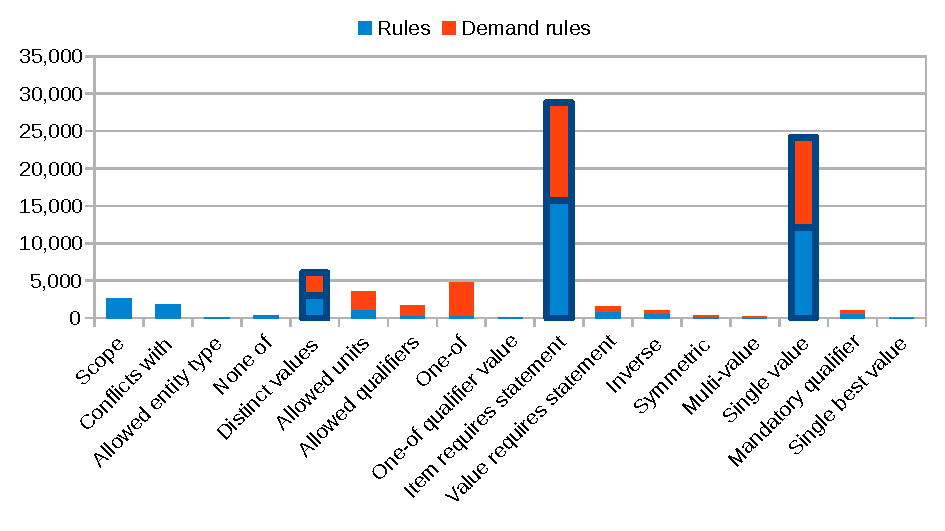
\includegraphics[width=\linewidth]{images/rules.pdf}
\caption{Number of rules and demanded rules}\label{fig_rules}
\end{figure}

\subsection{Facts}
Figure \ref{fig_facts} shows the number of facts loaded into VLog per constraint. Base facts denote those directly extracted from the JSON-Dump and corresponding to one of the predicates listed in Section \ref{subsec_representation}. Inequality are the letter\(_i\) facts created to establish inequality as described in Section \ref{sec_constraints_using_inequality}. Note that in the demanded (and encoded) mode, every entry for which inequality should be established is usually split into multiple letter\(_i\) facts based on its length, which is why the number of inequality facts can be up to ten times the number of base facts. Require facts list the order of statements or qualifiers as described in Section \ref{sec_constraints_using_statement_non}.

\begin{figure}
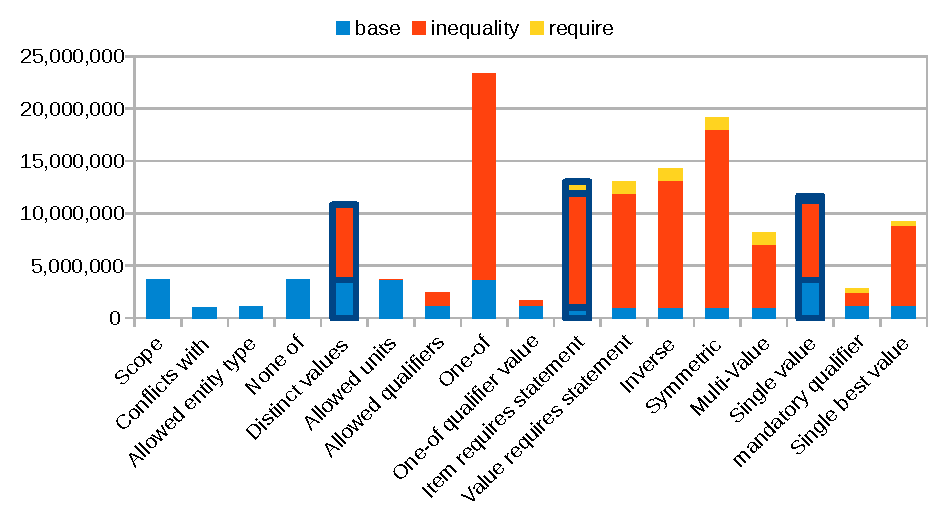
\includegraphics[width=\linewidth]{images/facts100,000.pdf}
\caption{Number of input facts per constraint}\label{fig_facts}
\end{figure}

The long runtimes of \emph{distinct values}, \emph{item requires statement} and \emph{single value} cannot be explained through the size of the input data. While all of them have more than 10 million input facts, this is also the case for other constraints that do not take nearly as much runtime. \emph{One-of}, \emph{symmetric} and \emph{inverse} have even more input facts than the three long-runtime constraints. The reason for the performance difference must be found elsewhere.

\subsection{Inequality evaluation}\label{sec_inequality_evaluation}
Inequality computation was implemented in three variants outlined in Section \ref{sec_constraints_using_inequality}: naive, encoded and demanded. Naive and encoded could not terminate for any dataset other than the smallest with 1,000 entities. Naive failed because the disk space needed for the precomputed inequality facts was not available. Encoded, while improving on the disk space needed, still failed due to out of memory errors. This behaviour is expected, since for an input of size \(n\) \(n^2\) inequalities have to be materialized. The runtimes for this dataset, presented in Figure \ref{fig_inequality}, shows a clear improvement when using the demanded approach. This shows that the overhead in rules introduced to enable the demanded approach, seen in Figure \ref{fig_rules}, is worth the improvements in performance gained through it.

\begin{figure}
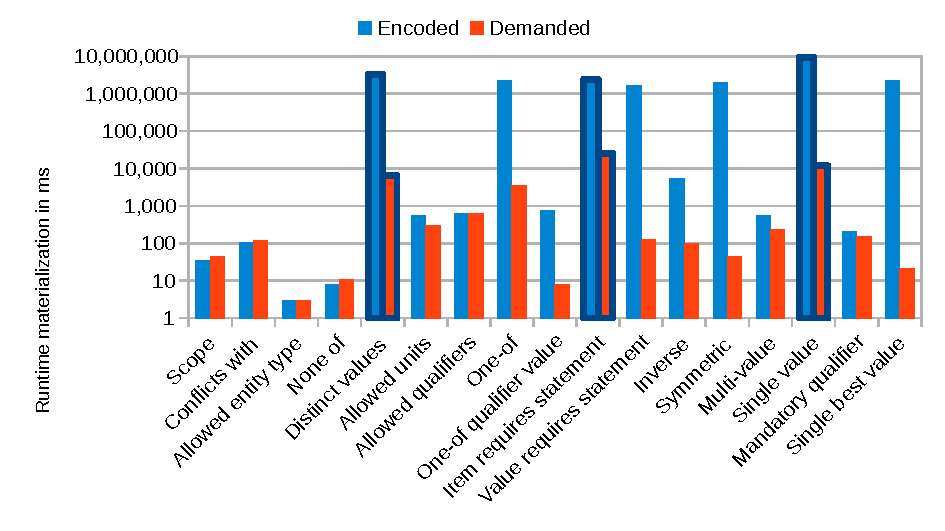
\includegraphics[width=\linewidth]{images/inequality1000.pdf}
\caption{Runtime materialization for 1,000 entities (encoded and demanded)}\label{fig_inequality}
\end{figure}

\subsection{Additional Derivations}
One possible bottleneck are the additional derivations necessary to identify violations. This includes the inequalities, demands for inequalities, requirements to determine statement non-existence as well as other helper rules introduced in Chapter \ref{cha_wikidata_constraints_explained}. Note that the four simple constraints described in Section \ref{sec_simple_constraints} do not generate any additional facts and are excluded from the chart. Figure \ref{fig_add_derivations} shows that the three performance-heavy constraints do generate by far the most additional derivations. The constraint with the smallest number of additional derivations, \emph{distinct values}, is almost an order of magnitude higher than the next highest, \emph{one-of}.

\begin{figure}
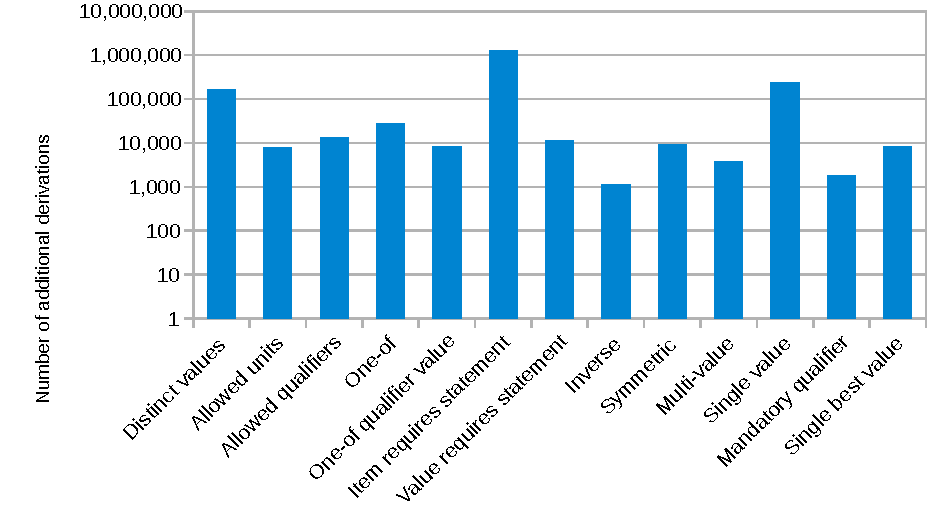
\includegraphics[width=\linewidth]{images/additionalDerivations100,000.pdf}
\caption{Additional derivations for 100,000 entities}\label{fig_add_derivations}
\end{figure}

\section{Findings}
Most constraints could be evaluated within a very short timeframe (< 1 minute). While the dataset does not include the entire database of Wikidata, which with 50m entities is about 500 times bigger, the runtimes for the entire dataset should still be within a reasonable frame. The exception are the three constraints focused on in Section \ref{sec_results}. As shown in that Section, the main difference between \emph{distinct values}, \emph{item requires statement}, and \emph{single value} and other constraints is
\begin{enumerate}[a)]
\item a larger amount of constrained properties (with a corresponding larger amount of rules) and
\item a larger amount of additional derivations
\end{enumerate}
The rules for these three constraints will now be analysed and possible reasons for this huge difference in performance outlined.

\subsection{Distinct values}
While the rules for the \emph{distinct values} constraint (see Section \ref{subsec_distinct_values}) are relatively simple in writing, they do require a large amount of processing. Distinct values requires the comparison of every constrained statement with every other constrained statement, meaning its evaluation would scale badly due to the quadratic growth of statements to be compared. Additionally, the number of inequalities that have to be evaluated according to the demanded approach (see Section \ref{sec_constraints_using_statement_non}) grows accordingly. Due to the nature of the constraint -- requiring distinct values for a property across all of Wikidata -- this is in all likelihood unavoidable.

\subsection{Item requires statement}\label{subsec_findings_item_requires_statement}
The \emph{item requires statement} constraint (see Section \ref{subsec_item_requires_statement}) creates additional facts about every statement on an entity with a constrained statement (if the constraint was violated on that entity). Of interest to note is that the \emph{value requires statement} constraint (see Section \ref{subsec_value_requires_statement}), which works almost identically, does not show a performance nearly as bad as \emph{item requires statement}. \emph{Value requires statement} has, however, only 244 constrained properties, while \emph{item requires statement} has 4265. This shows that the require approach scales badly with increasing number of require rules.

\subsection{Single value}
The \emph{single value} constraint (see Section \ref{subsec_single_value}) has to be analysed with regards to the two cases: without separators (Section \ref{subsubsec_single_value_no_separators}) and with separators (Section \ref{subsubsec_single_value_with_separators}.

\paragraph{No separators}
If no separators were given, the rules simply compare every statement on an entity with a constrained statement to said constrained statement. Since entity size does not increase with dataset size, this should not be the reason for \emph{single values} bad performance.

\paragraph{With separators}
The \emph{single value} constraint, like the \emph{item requires statement} constraint, uses a require approach to determine non-existence. For \emph{single value} this is qualifier non-existence on constrained statements. As seen in Section \ref{subsec_findings_item_requires_statement}, this could be a reason for the bad performance of the analysis for this constraint. Another source of processing time for \emph{single value} are the has\_same facts, which need to compare all constrained statements on the same item and all their qualifiers. Of interest to note is that the \emph{single best value} constraint (see Section \ref{subsec_single_best_value}) works in almost the same way but does not suffer from the same performance. Again, the number of constrained properties is significantly lower for \emph{single best value} (203) compared to \emph{single value} (2909).

\subsection{Possible adaptations}
Since the problematic performance of \emph{item requires statement} and \emph{single value} are not visible in \emph{value requires statement} and \emph{single best value}, which are very similar in their rule modelling, a possible adaptation would be to not evaluate all constrained properties for these constraints in bulk but split them into smaller sets, evaluating each set individually to combat the problematic scaling of the require pattern. The precomputed datasets could be kept, meaning only the reasoning step would have to be repeated.

\subsection{Adaptations to VLog}

\subsubsection{Sorting facts for column-based storage}
VLog uses a column-based storage format where the first column is fully sorted and all following columns are sorted w.r.t. the preceding column. These columns are then run-length encoded. To minimize memory requirements and maximize access speed, predicates should be sorted in such a way that each entry has a smaller number of unique constants than the next entry.

\begin{example}
The predicate \emph{statement\_EDB} lists the \emph{statement ID}, \emph{entity ID}, \emph{property ID} and \emph{value}. To optimize this for VLog, a new order must be created. \emph{property ID} should be the first entry, because there are only \todo{number of properties and link} different properties on Wikidata as of September 2018. The \emph{statement ID} needs to be moved to the last position since it is unique for all statements, meaning for any data source with \(n\) statements there would be \(n\) unique \emph{statement IDs}. Finally \emph{entity ID} should be before \emph{value}, because every \emph{entity ID} could also be a \emph{value}, but value can take additional string values.

The final, optimized order is then: \emph{property ID}, \emph{entity ID}, \emph{value}, \emph{statement ID}.
\end{example}

This order is, however, not easily readable and, if taken as presented, would likely cause implementation errors because the different positions are confused for each other. To prevent this the datasets imported from Wikidata and created during preprocessing as well as the rules outlined in Chapter \ref{cha_wikidata_constraints_explained} are sorted afterwards. Thus the rules can be kept in a readable form while still optimizing for VLog.

\subsubsection{Sorting conjunctions for left-to-right evaluation}
Conjunctions in VLog are evaluated from left to right, meaning the engine computes the matches of the first atom and, based on those findings, proceeds with the next atom. The rules as presented are not optimal regarding this process. Ideally, atoms should be sorted by the size of the intermediate results they incur. 

\subsubsection{Results}


\chapter{Conclusion}


\end{document}
